% !TeX program = xelatex
\documentclass[UTF8,zihao=-4]{ctexart}

\usepackage[a4paper,top=3cm,bottom=2.5cm,left=2.5cm,right=2.5cm,footskip=1.5cm]{geometry}
\usepackage{amsmath,amssymb,bm}
\usepackage{graphicx}
\usepackage{booktabs}
\usepackage{tabularx}
\usepackage{array}
\usepackage{float}
\usepackage{subcaption}
\usepackage{caption}
\usepackage{enumitem}
\usepackage{xcolor}
\usepackage{hyperref}
\usepackage{placeins}
\usepackage{etoolbox}
\usepackage{makecell}
\usepackage{tikz}
\usetikzlibrary{arrows.meta,positioning,fit,calc}

\graphicspath{{images/}}
\hypersetup{colorlinks=true,linkcolor=black,citecolor=black,urlcolor=black}
\renewcommand{\contentsname}{目\quad 录}

\ctexset{
  section = {
    format = \centering\zihao{3}\heiti,
    name = {},
    number = \arabic{section},
    aftername = \quad,
    beforeskip = 1.0em,
    afterskip = 1.0em
  },
  subsection = {
    format = \zihao{-3}\heiti,
    name = {},
    number = \thesection.\arabic{subsection},
    aftername = \quad,
    beforeskip = 0.8em,
    afterskip = 0.6em
  },
  subsubsection = {
    format = \zihao{4}\heiti,
    name = {},
    number = \thesubsection.\arabic{subsubsection},
    aftername = \quad,
    beforeskip = 0.6em,
    afterskip = 0.4em
  }
}

\setlength{\parindent}{2em}
\setlength{\parskip}{0pt}
\linespread{1.32}
\pagestyle{plain}
\setcounter{tocdepth}{2}
\setcounter{secnumdepth}{2}
\raggedbottom
\setlength{\floatsep}{0.25em plus 0.08em minus 0.08em}
\setlength{\textfloatsep}{0.28em plus 0.08em minus 0.08em}
\setlength{\intextsep}{0.25em plus 0.08em minus 0.08em}
\setlength{\abovecaptionskip}{0.2em}
\setlength{\belowcaptionskip}{-0.15em}
\renewcommand{\topfraction}{0.96}
\renewcommand{\bottomfraction}{0.92}
\renewcommand{\textfraction}{0.04}
\renewcommand{\floatpagefraction}{0.95}
\captionsetup{font={small,stretch=1.0},labelfont=bf,labelsep=quad,skip=0.18em}
\captionsetup[subfigure]{skip=0.12em}
\setlist[itemize]{leftmargin=2.5em,itemsep=0.2em}
\setlist[enumerate]{leftmargin=2.5em,itemsep=0.2em}
\Urlmuskip=0mu plus 2mu

\newcommand{\diff}{\mathrm{d}}
\newcommand{\norm}[1]{\left\lVert #1 \right\rVert}
\newcommand{\trans}{^{\mathsf T}}
\newcommand{\panelh}{0.105\textheight}
\newcommand{\widepanelh}{0.13\textheight}
\tikzset{
  flowbox/.style={draw=black!55, fill=blue!6, rounded corners=2pt, align=center, minimum height=0.85cm, text width=2.65cm, font=\small},
  modulebox/.style={draw=black!55, fill=green!7, rounded corners=2pt, align=center, minimum height=0.85cm, text width=2.75cm, font=\small},
  resultbox/.style={draw=black!55, fill=orange!10, rounded corners=2pt, align=center, minimum height=0.85cm, text width=2.65cm, font=\small},
  warnbox/.style={draw=black!55, fill=red!7, rounded corners=2pt, align=center, minimum height=0.85cm, text width=2.75cm, font=\small},
  flowarrow/.style={-Latex, thick, draw=black!60}
}
% Keep sections flowing to avoid sparse image-only pages.
\pretocmd{\section}{\clearpage}{}{}

\title{\bfseries 基于 MuJoCo 与 Rerun 的六自由度机械臂避障路径规划数值实验研究\\
\large 逆运动学数值解法与路径规划算法的对比分析}
\author{
工程数值分析课程论文\\[0.4em]
研究主题：机械臂逆运动学与避障路径规划\\
小组成员：洪竞权、贺禄文、周志鹏、鄢卓\\
重庆大学卓越工程师学院
}
\date{2026 年 5 月}

\begin{document}

\begin{titlepage}
  \thispagestyle{empty}
  \begin{center}
    \vspace*{0.45cm}
    {\zihao{4}\heiti 数值分析案例报告\par}
    \vspace{2.4cm}
    {\zihao{2}\heiti 基于 MuJoCo 与 Rerun 的六自由度机械臂\par}
    \vspace{0.45cm}
    {\zihao{2}\heiti 避障路径规划数值实验研究报告\par}
    \vspace{1.0cm}
    {\zihao{3}\heiti 逆运动学数值解法与路径规划算法的对比分析\par}
  \end{center}
  \vspace{2.0cm}
  \begin{center}
    {\zihao{3}\heiti
    \begin{tabular}{@{}>{\raggedleft\arraybackslash}p{4.0cm}@{\quad}p{8.2cm}@{}}
      小组成员： & 洪竞权\quad 贺禄文\quad 周志鹏\quad 鄢卓 \\
      学\quad 号： & 20234262\quad 20234232\quad 20230647\quad 20232695 \\
      班\quad 级： & 明月01班 \\
      指导老师： & 何光辉 \\
    \end{tabular}
    }
  \end{center}
  \vfill
  \begin{center}
    {\zihao{2}\heiti 重庆大学卓越工程师学院\par}
    \vspace{0.35cm}
    {\zihao{3}\heiti 2026年5月\par}
  \end{center}
\end{titlepage}

\pagenumbering{Roman}
\begingroup
  \zihao{-4}
  \setlength{\parskip}{0pt}
  \linespread{1.15}\selectfont
  \tableofcontents
  \thispagestyle{plain}
\endgroup
\newpage

\begin{center}
  {\zihao{3}\heiti 摘\quad 要\par}
\end{center}
\addcontentsline{toc}{section}{摘要}
\vspace{1em}
六自由度机械臂在工业装配、柔性制造和实验室自动化中需要同时满足目标到达、关节约束和避障安全。本文围绕工程数值分析课程要求，构建了一个基于 MuJoCo 与 Rerun 的机械臂数值实验平台，以 UR5e 类六自由度模型为对象，比较 Jacobian 伪逆法、阻尼最小二乘法、Levenberg--Marquardt 风格阻尼 Gauss--Newton 法和 SciPy 最小二乘基线，并进一步比较 RRT、RRT-Connect、PRM 与人工势场法在五类固定场景中的路径规划表现。论文重点不是展示单次动画，而是将机械臂问题拆解为非线性方程组求解、线性化迭代、构型空间搜索、离散碰撞检测、轨迹平滑与数值差分评价等可复现实验环节。实验每个算法在每个场景下重复 50 次，并导出 CSV 数据、统计汇总和论文图表。结果显示，SciPy 基线末端误差最低但耗时更高；阻尼 Jacobian 方法在精度和速度之间较均衡；RRT-Connect 在当前五类场景中保持 100\% 成功率，并在综合评分上整体占优；人工势场法在无障碍和近奇异场景有效，但在单障碍、多障碍和窄通道场景中容易受局部极小值限制。上述结果说明，数值稳定性、采样策略和碰撞检测分辨率共同决定机械臂避障规划的可用性\cite{siciliano2009robotics,lavalle2006planning}。

\noindent{\heiti 关键词：}六自由度机械臂；MuJoCo；Rerun；逆运动学；阻尼最小二乘；RRT-Connect；路径规划；数值实验
\newpage

\pagenumbering{arabic}
\section{引言与课程问题映射}

\subsection{工程背景}
机械臂避障路径规划看似是机器人应用问题，本质上包含多个数值计算子问题。目标点到关节角的映射需要求解非线性方程组；障碍物规避需要在高维构型空间中搜索可行路径；离散路径需要平滑和重采样；轨迹质量又要通过差分、范数、路径长度和安全距离统计进行评价。相比只展示仿真动画，本文更强调“模型、算法、数据、图表”之间的闭环。

本文采用 MuJoCo 进行多刚体正运动学、几何距离和碰撞检测\cite{todorov2012mujoco}，使用 Rerun 记录三维轨迹与关节序列\cite{rerunDocs2024}，并用 Matplotlib 导出 LaTeX 可引用图表。实验固定随机种子、起始构型、目标点、障碍物和算法参数，使每个结论都能回溯到 CSV 记录。

\begin{equation}
  \text{工程任务}
  \quad\Longrightarrow\quad
  \text{数值建模}
  \quad\Longrightarrow\quad
  \text{程序实验}
  \quad\Longrightarrow\quad
  \text{统计评价}.
  \label{eq:workflow}
\end{equation}

\subsection{课程知识点对应关系}
本文把机械臂避障任务映射到工程数值分析中的五类知识点。非线性方程组求解对应逆运动学；线性方程组求解对应每步 Jacobian 线性化；插值和平滑对应规划路径后处理；数值微分对应速度、加速度和 jerk 指标；条件数分析对应近奇异位形的稳定性解释。

\begin{table}[!htbp]
  \centering
  \caption{机械臂任务与数值分析知识点的对应关系}
  \label{tab:course-map}
  \begin{tabularx}{\textwidth}{p{3.6cm}X p{3.2cm}}
    \toprule
    工程环节 & 数值形式 & 主要输出 \\
    \midrule
    目标点到达 & 非线性方程组 $f(\bm q)-\bm p_d=\bm 0$ & IK 误差、迭代次数 \\
    Jacobian 迭代 & 最小二乘或阻尼线性系统 & 条件数、耗时 \\
    避障规划 & 构型空间采样与离散边检测 & 成功率、路径长度 \\
    轨迹执行 & 路径平滑、重采样与差分 & 速度、加速度、jerk \\
    安全评价 & 几何体距离的采样近似 & 最小安全距离 \\
    \bottomrule
  \end{tabularx}
\end{table}

\subsection{实验场景与研究目标}
实验包含六个基准或过渡场景，并以 \texttt{scene\_pass\_through\_maze} 作为综合展示场景。基准场景用于比较不同 IK 方法和规划器在常规障碍分布下的统计表现；混合迷宫场景用于连接窄通道和小框插入两类难题；综合展示场景使用 MuJoCo Menagerie 中的完整 UR5e MJCF 模型，强调末端在密集悬浮障碍中插入小框目标的空间效果。研究目标包括两个层面：第一，比较不同 IK 方法在精度、耗时和条件数上的差异；第二，比较不同规划器在成功率、效率、路径质量、安全距离和地面可执行性上的差异。

\begin{table}[!htbp]
  \centering
  \caption{实验场景}
  \label{tab:scenes}
  \begin{tabularx}{\textwidth}{p{3.6cm}p{3.5cm}X}
    \toprule
    场景 & 目标点 / m & 障碍物说明 \\
    \midrule
    S0 无障碍 & $(0.55,0.18,0.44)$ & 原始编号 scene\_00\_no\_obstacle，用于验证目标到达能力。\\
    S1 单障碍 & $(0.47,0.22,0.42)$ & 原始编号 scene\_01\_single\_box，包含单个 box。\\
    S2 多障碍 & $(0.42,-0.28,0.48)$ & 原始编号 scene\_02\_multi\_obstacles，包含 box、sphere、cylinder。\\
    S3 窄通道 & $(0.62,0.02,0.43)$ & 原始编号 scene\_03\_narrow\_passage，两侧墙体与顶部球体构成通道。\\
    S4 近奇异 & $(0.76,-0.06,0.48)$ & 原始编号 scene\_04\_near\_singularity，目标接近伸展位形。\\
    S5 混合迷宫 & $(0.55,0.03,0.43)$ & 原始编号 scene\_05\_mixed\_maze\_passage，包含多组门洞和偏置障碍。\\
    S6 小框插入 & $(0.62,0.02,0.43)$ & 综合展示编号 scene\_pass\_through\_maze，包含目标小框和密集悬浮障碍。\\
    \bottomrule
  \end{tabularx}
\end{table}

图 \ref{fig:mujoco-scenes} 给出了由 MuJoCo 离屏渲染直接生成的场景截图。截图保留了仿真模型中的地面、机械臂胶囊连杆和障碍物几何体，用于说明后续 CSV 指标并非脱离空间场景的抽象数值。

\begin{figure}[!htbp]
  \centering
  \begin{subfigure}{0.32\textwidth}
    \centering
    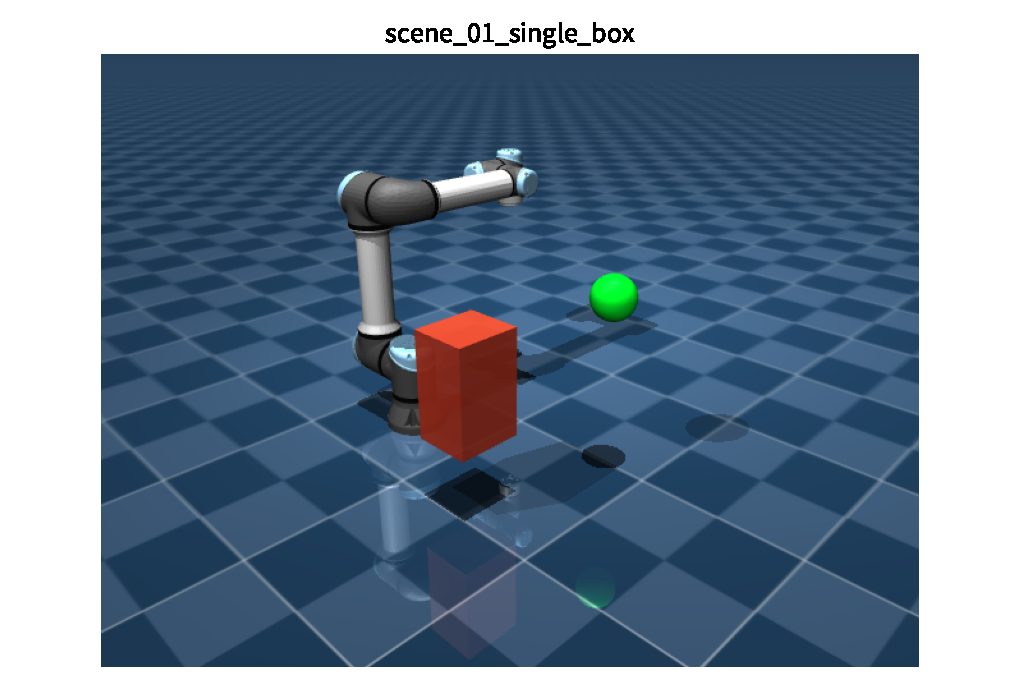
\includegraphics[width=\linewidth,height=0.13\textheight,keepaspectratio]{generated/mujoco_scene_scene_01_single_box.pdf}
    \caption{单障碍场景}
  \end{subfigure}
  \hfill
  \begin{subfigure}{0.32\textwidth}
    \centering
    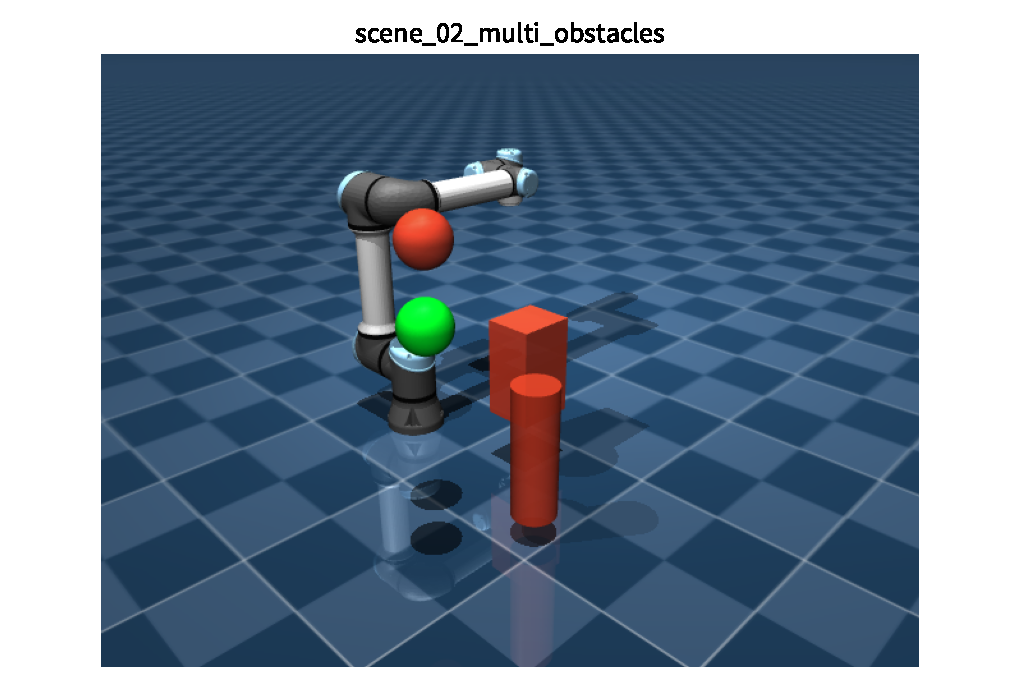
\includegraphics[width=\linewidth,height=0.13\textheight,keepaspectratio]{generated/mujoco_scene_scene_02_multi_obstacles.pdf}
    \caption{多障碍场景}
  \end{subfigure}
  \hfill
  \begin{subfigure}{0.32\textwidth}
    \centering
    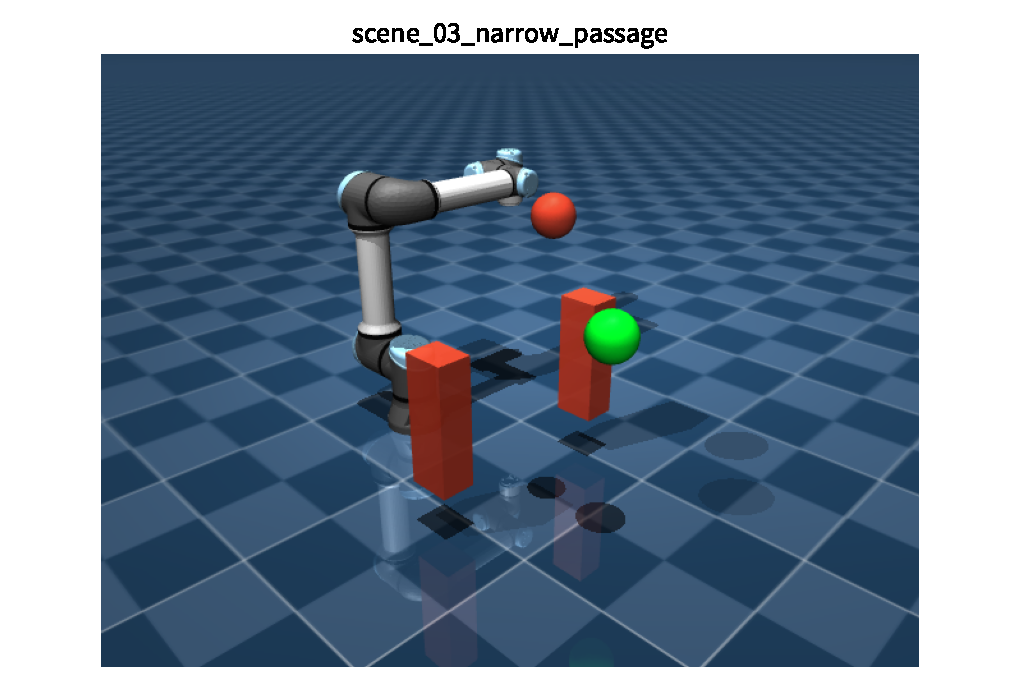
\includegraphics[width=\linewidth,height=0.13\textheight,keepaspectratio]{generated/mujoco_scene_scene_03_narrow_passage.pdf}
    \caption{窄通道场景}
  \end{subfigure}
  \caption{MuJoCo 离屏渲染得到的真实仿真场景截图。蓝色胶囊表示机械臂连杆，红色几何体表示障碍物。}
  \label{fig:mujoco-scenes}
\end{figure}

主展示场景使用 MuJoCo Menagerie 的完整 UR5e 模型，模型文件采用仓库中的 UR5e \texttt{scene.xml}，末端 site 为 \texttt{attachment\_site}。关键参数列于表 \ref{tab:main-scene-params}。障碍物由一个插入式小框和 8 个悬浮 box 组成，小框开口约为 $0.50\times0.34$ m，目标位于小框开口附近的后方，使可行轨迹呈现末端插入框内的效果。该场景同时把地面作为硬约束：任何路径点或边插值点发生地面穿透，均不计为成功。

\begin{table}[!htbp]
  \centering
  \caption{主展示场景关键参数}
  \label{tab:main-scene-params}
  \small
  \begin{tabularx}{\textwidth}{p{3.8cm}X}
    \toprule
    参数 & 数值或说明 \\
    \midrule
    模型文件 & \path{third_party/mujoco_menagerie/universal_robots_ur5e/scene.xml} \\
    起始构型 / rad & $[-1.5708,-1.5708,1.5708,-1.5708,-1.5708,0]$ \\
    目标位置 / m & $(0.62,0.02,0.43)$ \\
    目标姿态四元数 & $[0.44614,0.282258,0.366804,0.765993]$，格式为 $wxyz$ \\
    障碍布局 & 1 个插入式小框 + 8 个悬浮 box + 地面 plane \\
    成功硬约束 & 无障碍碰撞，且地面间隙不小于 $-10^{-4}$ m \\
    \bottomrule
  \end{tabularx}
\end{table}

\subsection{仿真环境与场景设计}
仿真环境由机器人模型、几何约束、目标位姿和随机性控制四部分组成。MuJoCo 负责根据 MJCF 文件计算正运动学、site 位姿、几何体距离和接触关系；配置文件负责固定关节名称、起始构型、目标位置姿态和算法参数。与只使用简化连杆模型不同，主展示场景直接加载完整 UR5e Menagerie 模型\cite{mujocoMenagerie2024}，因此碰撞检测需要同时识别未显式命名的机器人 collision geom、地面 plane 和动态注入的障碍物 geom。

图 \ref{fig:scene-design-blocks} 用方块图概括主场景的组成。目标小框提供局部穿越约束，悬浮障碍提供中前段扰动，地面 plane 提供可执行性边界；目标位置和目标姿态共同决定末端最终插入方向。这样的设计使算法既要完成目标到达，又要避免把穿地或穿障轨迹误判为成功。

\begin{figure}[!htbp]
  \centering
  \begin{tikzpicture}[node distance=0.85cm and 0.8cm]
    \node[modulebox] (robot) {完整 UR5e\\Menagerie MJCF};
    \node[modulebox, right=of robot] (ground) {地面 plane\\$d_g(\bm q)$ 约束};
    \node[modulebox, right=of ground] (frame) {目标小框\\插入式 aperture};
    \node[modulebox, below=of ground] (floats) {8 个悬浮 box\\密集避障扰动};
    \node[modulebox, left=of floats] (pose) {目标位置 + 姿态\\$\bm p_d,\bm s_d$};
    \node[resultbox, right=of floats] (scene) {主展示场景\\pass-through maze};
    \draw[flowarrow] (robot) -- (ground);
    \draw[flowarrow] (ground) -- (frame);
    \draw[flowarrow] (pose) -- (floats);
    \draw[flowarrow] (frame) -- (scene);
    \draw[flowarrow] (floats) -- (scene);
  \end{tikzpicture}
  \caption{主仿真场景的方块式组成。机器人模型、地面、小框、悬浮障碍和目标位姿共同定义可行路径空间。}
  \label{fig:scene-design-blocks}
\end{figure}

\begin{figure}[!htbp]
  \centering
  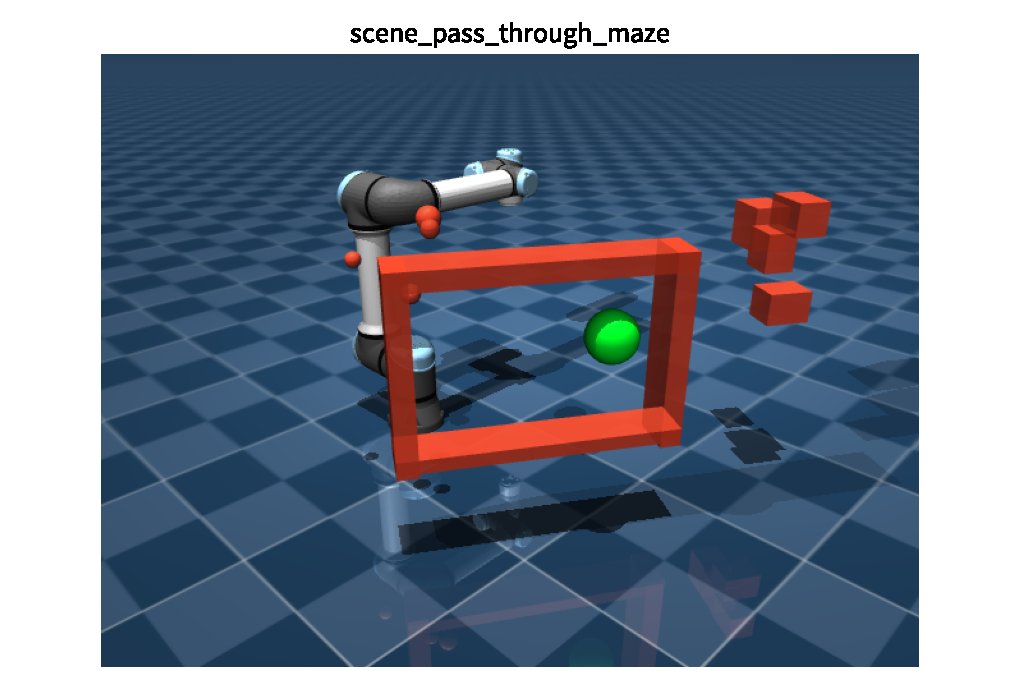
\includegraphics[width=0.76\linewidth,height=0.22\textheight,keepaspectratio]{generated/mujoco_scene_scene_pass_through_maze.pdf}
  \caption{主展示场景 \texttt{scene\_pass\_through\_maze}。完整 UR5e 模型、目标小框、密集悬浮障碍和地面共同构成末端插入式避障任务。}
  \label{fig:pass-through-scene}
\end{figure}

\section{机械臂运动学建模}

\subsection{关节空间与任务空间}
设六自由度机械臂关节变量为
\begin{equation}
  \bm q=
  \begin{bmatrix}
  q_1&q_2&q_3&q_4&q_5&q_6
  \end{bmatrix}\trans .
  \label{eq:q-vector}
\end{equation}

正运动学将关节空间映射到末端位置空间：
\begin{equation}
  f:\mathbb{R}^{6}\rightarrow\mathbb{R}^{3}.
  \label{eq:fk-map}
\end{equation}

给定目标末端位置 $\bm p_d$，位置残差定义为
\begin{equation}
  \bm r(\bm q)=f(\bm q)-\bm p_d .
  \label{eq:ik-residual}
\end{equation}

逆运动学的核心目标是寻找使残差范数足够小的关节构型：
\begin{equation}
  \bm q^\star=\arg\min_{\bm q}\frac{1}{2}\norm{\bm r(\bm q)}_2^2 .
  \label{eq:ik-objective}
\end{equation}

考虑关节限位后，优化问题变为
\begin{equation}
  \bm q_{\min}\leq \bm q\leq \bm q_{\max}.
  \label{eq:joint-limit}
\end{equation}

基础场景以位置目标为主；主展示场景进一步给出目标姿态。若目标四元数为 $\bm s_d$，当前末端四元数为 $\bm s(\bm q)$，则姿态误差用相对旋转向量 $\bm e_R(\bm q)$ 表示。此时 IK 残差写成
\begin{equation}
  \bm r_{\mathrm{pose}}(\bm q)=
  \begin{bmatrix}
    f(\bm q)-\bm p_d\\
    w_R\bm e_R(\bm q)
  \end{bmatrix},
  \label{eq:pose-residual}
\end{equation}
其中 $w_R$ 为姿态权重。没有给出目标姿态时，残差退化为位置误差。

\subsection{Jacobian 线性化}
非线性最小二乘问题不能直接用一次线性方程求解，因此各类 Jacobian 方法都采用“局部线性化--求增量--更新构型”的迭代框架。在当前迭代点 $\bm q_k$ 附近，正运动学可一阶展开为
\begin{equation}
  f(\bm q_k+\Delta\bm q)
  \approx
  f(\bm q_k)+J(\bm q_k)\Delta\bm q .
  \label{eq:linearization}
\end{equation}

令目标误差为
\begin{equation}
  \bm e_k=\bm p_d-f(\bm q_k),
  \label{eq:error-vector}
\end{equation}

则线性化子问题写成
\begin{equation}
  J(\bm q_k)\Delta\bm q_k\approx \bm e_k .
  \label{eq:linear-system}
\end{equation}

也就是说，每一步 IK 都把原来的非线性目标临时替换成一个线性最小二乘问题：
\begin{equation}
  \Delta\bm q_k
  =
  \arg\min_{\Delta\bm q}
  \frac{1}{2}\norm{J(\bm q_k)\Delta\bm q-\bm e_k}_2^2 .
  \label{eq:ik-local-ls}
\end{equation}
求得 $\Delta\bm q_k$ 后，再用步长 $\eta$ 更新关节角。该过程的数值质量取决于两个因素：一是一阶近似是否足够准确，二是矩阵 $J$ 是否接近奇异。前者受步长影响，后者由奇异值分布和条件数反映。

Jacobian 条件数用于衡量线性化敏感性：
\begin{equation}
  \kappa(J)=\frac{\sigma_{\max}(J)}{\sigma_{\min}(J)} .
  \label{eq:condition}
\end{equation}

当 $\sigma_{\min}(J)$ 较小时，微小末端误差可能放大成较大的关节增量，近奇异场景因此更容易出现数值不稳定。

\subsection{构型空间与碰撞检测}
规划器在关节空间中寻找离散路径
\begin{equation}
  \Pi=\{\bm q_0,\bm q_1,\ldots,\bm q_N\},
  \label{eq:path}
\end{equation}

其中
\begin{equation}
  \bm q_0=\bm q_s,\qquad \bm q_N=\bm q_g .
  \label{eq:path-boundary}
\end{equation}

自由空间定义为
\begin{equation}
  \mathcal C_{\mathrm{free}}
  =
  \{\bm q\mid d_{\min}(\bm q)>0,\ d_g(\bm q)\geq -10^{-4},\ \bm q_{\min}\leq \bm q\leq \bm q_{\max}\}.
  \label{eq:c-free}
\end{equation}

相邻节点之间采用线性插值做边检测：
\begin{equation}
  \bm q(\alpha)=(1-\alpha)\bm q_i+\alpha\bm q_{i+1},
  \qquad
  \alpha\in[0,1].
  \label{eq:edge-interp}
\end{equation}

连续边被离散采样近似：
\begin{equation}
  \alpha_m=\frac{m}{M},\qquad m=0,1,\ldots,M .
  \label{eq:edge-sample}
\end{equation}

本文固定边检测分辨率为 $0.06$ rad，使不同规划器在相同安全近似条件下比较。

\section{逆运动学数值解法推导}

\subsection{Jacobian 伪逆法}
对于欠定线性系统 $J\Delta\bm q=\bm e$，伪逆法给出最小范数解\cite{buss2004ik}：
\begin{equation}
  \Delta\bm q_k=J(\bm q_k)^+\bm e_k .
  \label{eq:pinv-update}
\end{equation}

若 $J$ 行满秩，则
\begin{equation}
  J^+=J\trans(JJ\trans)^{-1}.
  \label{eq:pinv-form}
\end{equation}

更新公式为
\begin{equation}
  \bm q_{k+1}=\bm q_k+\eta\Delta\bm q_k .
  \label{eq:ik-update}
\end{equation}

其中 $\eta$ 为步长缩放系数。伪逆法的优点是形式直接、计算量小，在远离奇异位形时能快速降低位置误差；缺点是没有显式惩罚过大的关节增量。当 $JJ\trans$ 接近奇异时，较小的任务空间误差也可能被放大成较大的 $\Delta\bm q$，从而引起振荡或接近关节限位。因此本文把条件数作为 IK 结果的重要伴随指标，而不是只报告末端误差。

\subsection{阻尼最小二乘法}
阻尼最小二乘法把关节增量写成正则化最小二乘问题\cite{wampler1986dls,nakamura1986singularity}：
\begin{equation}
  \Delta\bm q_k
  =
  \arg\min_{\Delta\bm q}
  \left(
  \norm{J\Delta\bm q-\bm e_k}_2^2
  +
  \lambda^2\norm{\Delta\bm q}_2^2
  \right).
  \label{eq:dls-objective}
\end{equation}

对目标函数求导并令梯度为零：
\begin{equation}
  J\trans(J\Delta\bm q-\bm e_k)+\lambda^2\Delta\bm q=\bm 0 .
  \label{eq:dls-grad}
\end{equation}

得到正规方程：
\begin{equation}
  (J\trans J+\lambda^2I)\Delta\bm q=J\trans\bm e_k .
  \label{eq:dls-normal}
\end{equation}

等价地，在任务空间中可写为
\begin{equation}
  \Delta\bm q_k
  =
  J\trans(JJ\trans+\lambda^2I)^{-1}\bm e_k .
  \label{eq:dls-update}
\end{equation}

阻尼项 $\lambda^2I$ 提高了矩阵可逆性，代价是引入更保守的步长。从优化角度看，DLS 在降低末端误差的同时限制关节增量范数；从数值角度看，阻尼项抬高了正规方程矩阵的最小特征值，使近奇异时的求解更加平滑。若 $\lambda$ 过小，算法退化为接近伪逆法；若 $\lambda$ 过大，更新方向过于保守，可能需要更多迭代才能达到同样精度。

\subsection{LM 风格阻尼 Gauss--Newton}
LM 方法从非线性最小二乘目标出发\cite{levenberg1944least,marquardt1963algorithm}：
\begin{equation}
  \phi(\bm q)=\frac{1}{2}\norm{\bm r(\bm q)}_2^2 .
  \label{eq:lm-objective}
\end{equation}

Gauss--Newton 近似 Hessian 为
\begin{equation}
  H_k\approx J_k\trans J_k .
  \label{eq:gn-hessian}
\end{equation}

加入阻尼后，线性子问题为
\begin{equation}
  (J_k\trans J_k+\lambda_k I)\Delta\bm q_k=-J_k\trans\bm r_k .
  \label{eq:lm-system}
\end{equation}

若当前线性化可靠，则减小阻尼：
\begin{equation}
  \lambda_{k+1}<\lambda_k .
  \label{eq:lm-decrease}
\end{equation}

若误差下降不明显，则增大阻尼：
\begin{equation}
  \lambda_{k+1}>\lambda_k .
  \label{eq:lm-increase}
\end{equation}

因此 LM 风格方法可以在 Gauss--Newton 的快速收敛和梯度下降的稳健性之间折中。本文实现中固定了阻尼初值和迭代上限，使四类 IK 方法在同一目标位姿、同一起点和同一碰撞约束下比较。对于含姿态目标的主展示场景，残差向量同时包含位置误差与加权姿态误差；对于无姿态目标的基准场景，残差自动退化为三维位置误差。SciPy 最小二乘基线采用成熟数值优化库作为离线精度参照\cite{virtanen2020scipy}。

\begin{figure}[!htbp]
  \centering
  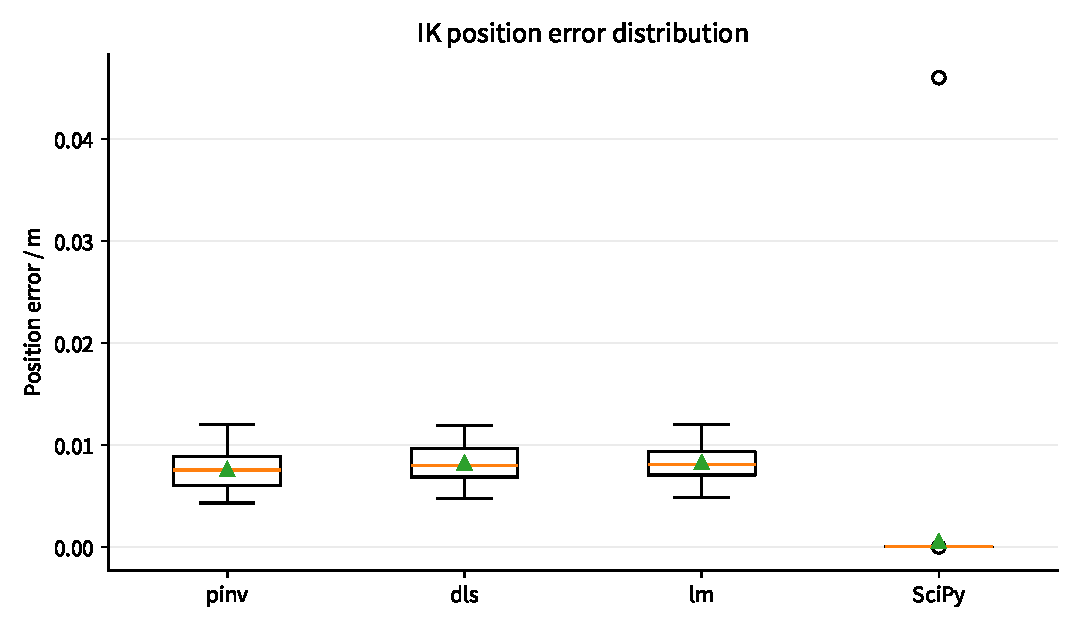
\includegraphics[width=0.86\linewidth,height=0.28\textheight,keepaspectratio]{generated/ik_error_boxplot.pdf}
  \caption{四类 IK 方法的末端位置误差分布。该图用于比较不同数值求解器的最终到达精度。}
  \label{fig:ik-error-boxplot}
\end{figure}

\begin{figure}[!htbp]
  \centering
  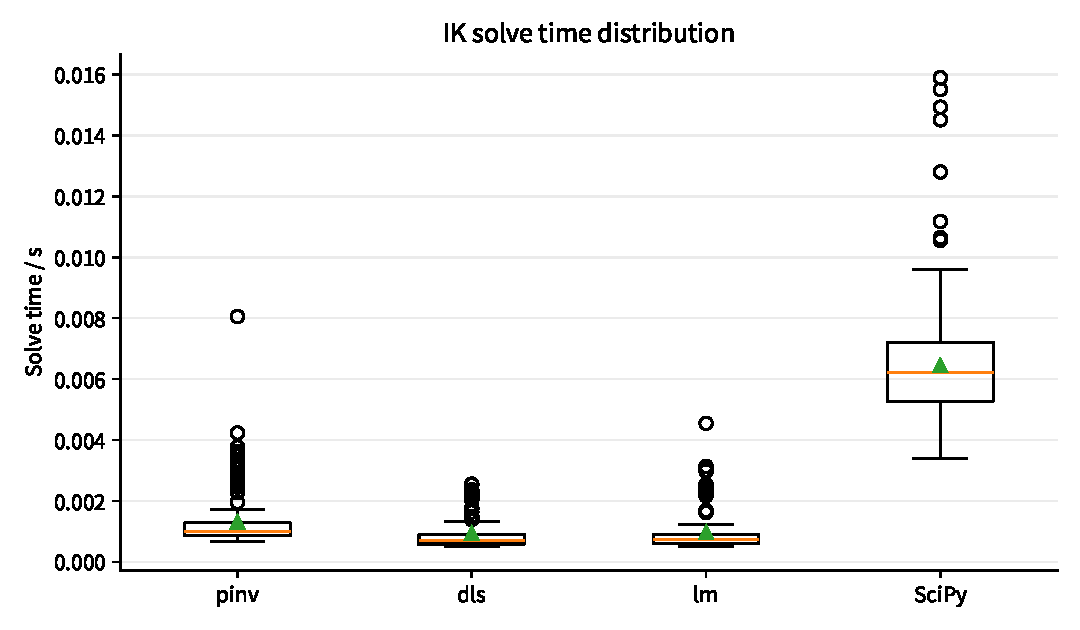
\includegraphics[width=0.86\linewidth,height=0.28\textheight,keepaspectratio]{generated/ik_time_boxplot.pdf}
  \caption{四类 IK 方法的求解耗时分布。SciPy 基线精度较高，但耗时明显高于三类 Jacobian 迭代法。}
  \label{fig:ik-time-boxplot}
\end{figure}

\begin{figure}[!htbp]
  \centering
  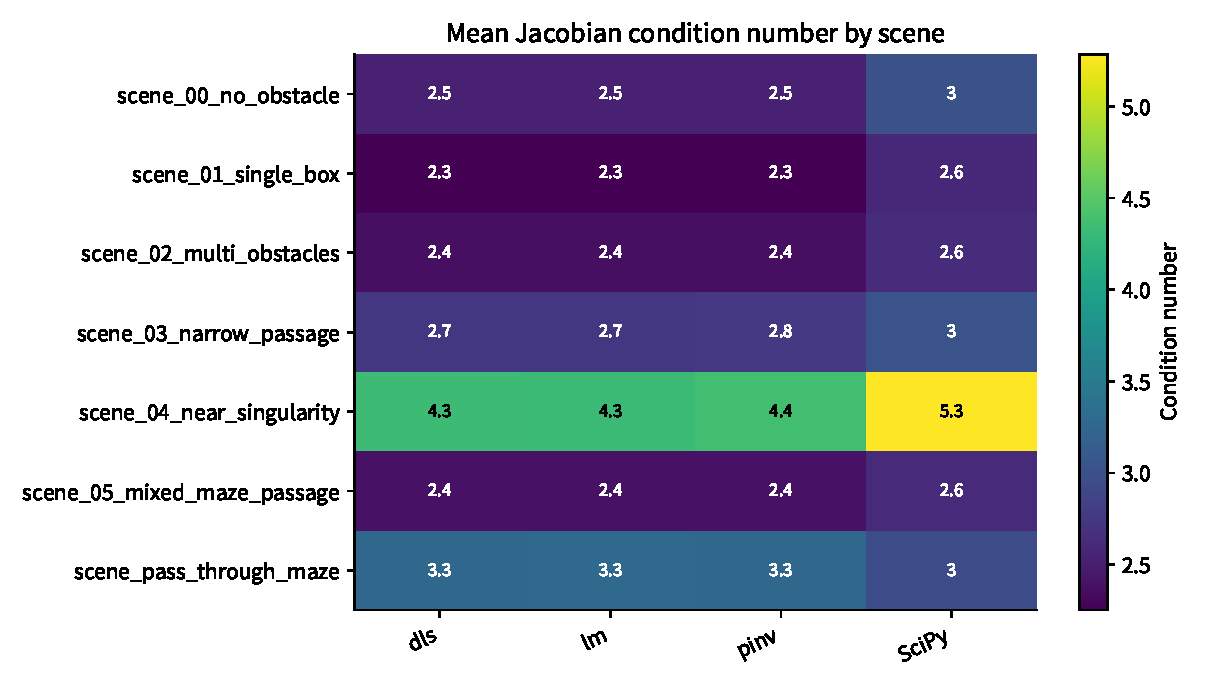
\includegraphics[width=0.86\linewidth,height=0.30\textheight,keepaspectratio]{generated/ik_condition_heatmap.pdf}
  \caption{不同场景和 IK 方法下的 Jacobian 条件数热力图。条件数越高，线性化子问题越容易放大末端误差。}
  \label{fig:ik-condition-heatmap}
\end{figure}

\begin{figure}[!htbp]
  \centering
  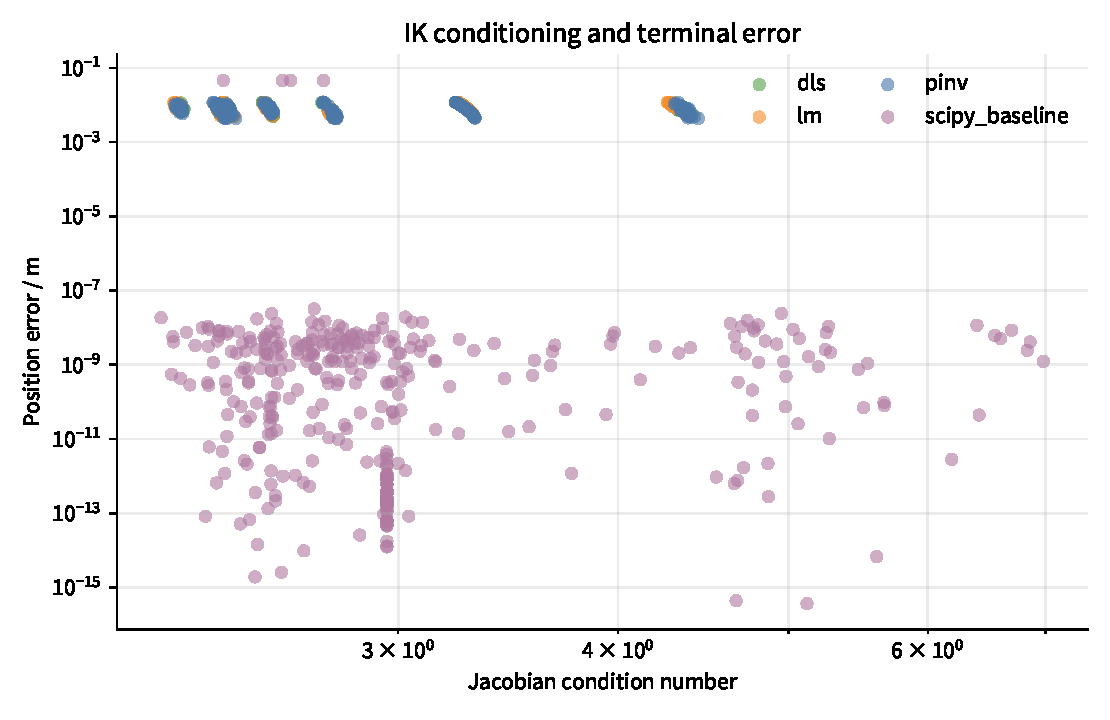
\includegraphics[width=0.86\linewidth,height=0.30\textheight,keepaspectratio]{generated/ik_condition_error_scatter.pdf}
  \caption{Jacobian 条件数与末端位置误差的关系。该图用于观察近奇异位形下数值敏感性对 IK 精度的影响。}
  \label{fig:ik-condition-error-scatter}
\end{figure}

\section{避障路径规划算法推导}

\subsection{RRT 与 RRT-Connect}
RRT 从起点树 $\mathcal T$ 出发，在关节空间随机采样\cite{lavalle2006planning}：
\begin{equation}
  \bm q_{\mathrm{rand}}\sim \mathcal U(\bm q_{\min},\bm q_{\max}) .
  \label{eq:rrt-sample}
\end{equation}

寻找树中最近节点：
\begin{equation}
  \bm q_{\mathrm{near}}
  =
  \arg\min_{\bm q\in\mathcal T}
  \norm{\bm q-\bm q_{\mathrm{rand}}}_2 .
  \label{eq:rrt-near}
\end{equation}

按固定步长扩展：
\begin{equation}
  \bm q_{\mathrm{new}}
  =
  \bm q_{\mathrm{near}}
  +
  s\frac{\bm q_{\mathrm{rand}}-\bm q_{\mathrm{near}}}
  {\norm{\bm q_{\mathrm{rand}}-\bm q_{\mathrm{near}}}_2}.
  \label{eq:rrt-steer}
\end{equation}

若边满足
\begin{equation}
  \bm q(\alpha)\in\mathcal C_{\mathrm{free}},
  \qquad
  \forall \alpha_m ,
  \label{eq:edge-valid}
\end{equation}

则把新节点加入树。一次 RRT 迭代可以概括为：采样随机点、寻找最近节点、按步长扩展、对扩展边做离散碰撞检测、把有效节点加入树。若新节点与目标构型的距离小于阈值，且最后一段边也满足式 \eqref{eq:edge-valid}，则规划成功。由于采样具有随机性，RRT 在窄通道或密集障碍中可能长时间无法采到有用的中间构型。

RRT-Connect 同时从起点和目标生长两棵树\cite{kuffner2000rrtconnect}：
\begin{equation}
  \mathcal T_s\leftrightarrow \mathcal T_g .
  \label{eq:rrt-connect-trees}
\end{equation}

每次迭代中，一棵树先向随机采样点扩展，另一棵树再尝试向新节点连续连接。当两棵树的扩展端点可以无碰撞连接时，路径即由两棵树拼接得到。双向搜索把单树“从起点摸索到目标”的问题变成“两端同时寻找连接点”的问题，因此在本文实验中明显减少了规划时间和碰撞检测次数。

\subsection{PRM 与人工势场法}
PRM 先采样构图，再在图上查询\cite{kavraki1996prm}。其计算过程分为三个阶段：首先在关节空间中采样候选节点并过滤掉无效状态；然后对每个节点寻找若干近邻，并用式 \eqref{eq:edge-valid} 判断边是否可行；最后在构造好的路线图上查询从起点到目标的最短路。可行节点集合为
\begin{equation}
  V=\{\bm q_i\mid \bm q_i\in\mathcal C_{\mathrm{free}}\}.
  \label{eq:prm-v}
\end{equation}

若两个节点足够近且边无碰撞，则添加边：
\begin{equation}
  E=\{(\bm q_i,\bm q_j)\mid \norm{\bm q_i-\bm q_j}_2<\rho,\ \overline{\bm q_i\bm q_j}\subset\mathcal C_{\mathrm{free}}\}.
  \label{eq:prm-e}
\end{equation}

查询阶段在图 $G=(V,E)$ 上求最短路：
\begin{equation}
  \Pi^\star=\arg\min_{\Pi\subset G}\sum_i\norm{\bm q_{i+1}-\bm q_i}_2 .
  \label{eq:prm-shortest}
\end{equation}

人工势场法把目标吸引和障碍排斥组合成势函数\cite{khatib1986real}：
\begin{equation}
  U(\bm q)=U_{\mathrm{att}}(\bm q)+U_{\mathrm{rep}}(\bm q).
  \label{eq:apf-total}
\end{equation}

吸引势可写为
\begin{equation}
  U_{\mathrm{att}}(\bm q)=\frac{1}{2}k_a\norm{\bm q-\bm q_g}_2^2 .
  \label{eq:apf-att}
\end{equation}

排斥势在障碍邻域内生效：
\begin{equation}
  U_{\mathrm{rep}}(\bm q)
  =
  \frac{1}{2}k_r
  \left(
  \frac{1}{d(\bm q)}-\frac{1}{d_0}
  \right)^2 ,
  \qquad d(\bm q)<d_0 .
  \label{eq:apf-rep}
\end{equation}

迭代方向由负梯度给出：
\begin{equation}
  \bm q_{k+1}
  =
  \bm q_k-\alpha\nabla U(\bm q_k).
  \label{eq:apf-update}
\end{equation}

APF 不显式构造全局路线图，而是根据当前构型处的势函数梯度不断更新。它的计算轻量、实现简单，在无障碍场景中通常能快速靠近目标；但排斥势和吸引势叠加后可能形成局部极小值，使梯度接近零：
\begin{equation}
  \norm{\nabla U(\bm q_k)}_2\approx 0,\qquad \bm q_k\neq \bm q_g .
  \label{eq:apf-local-min}
\end{equation}

这正是它在单障碍、多障碍和窄通道场景中失败的主要原因。本文把规划失败保留为实验结果，而不是简单丢弃：失败路径可以揭示采样图未连通、局部极小值、迭代上限和后处理无效等不同机制。

\begin{figure}[!htbp]
  \centering
  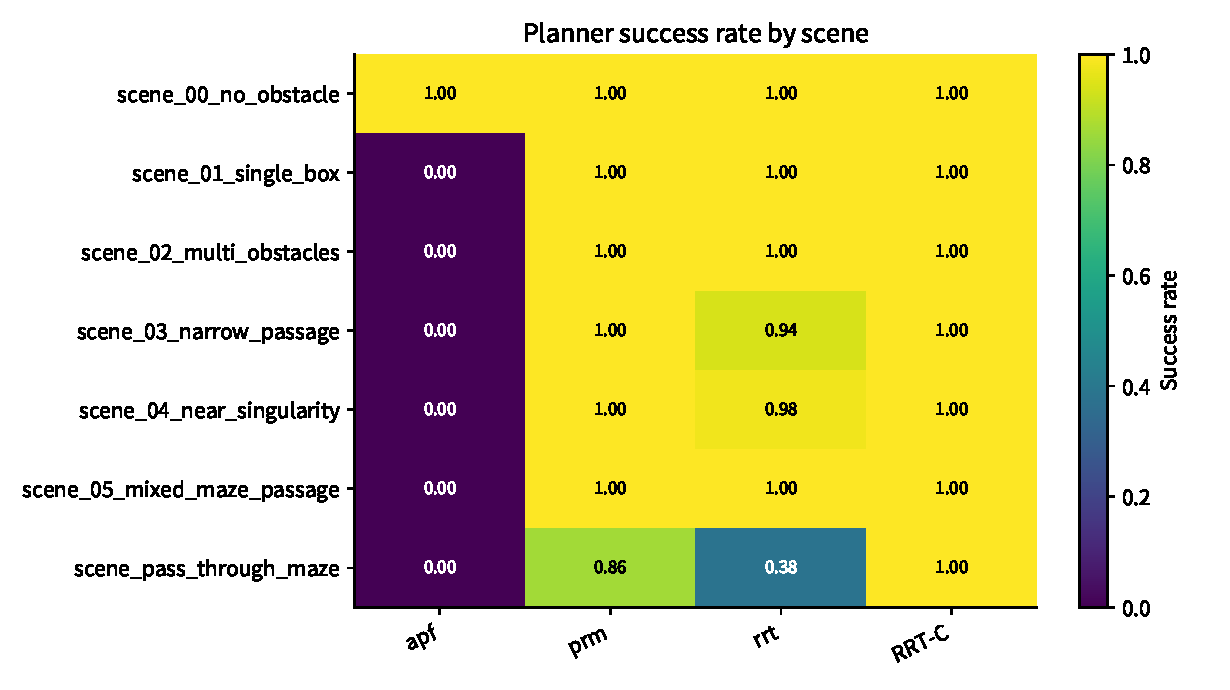
\includegraphics[width=0.86\linewidth,height=0.30\textheight,keepaspectratio]{generated/planner_success_heatmap.pdf}
  \caption{不同规划器在各场景中的成功率热力图。该图用于比较采样式规划和势场法在不同障碍复杂度下的可达性。}
  \label{fig:planner-success-heatmap}
\end{figure}

\begin{figure}[!htbp]
  \centering
  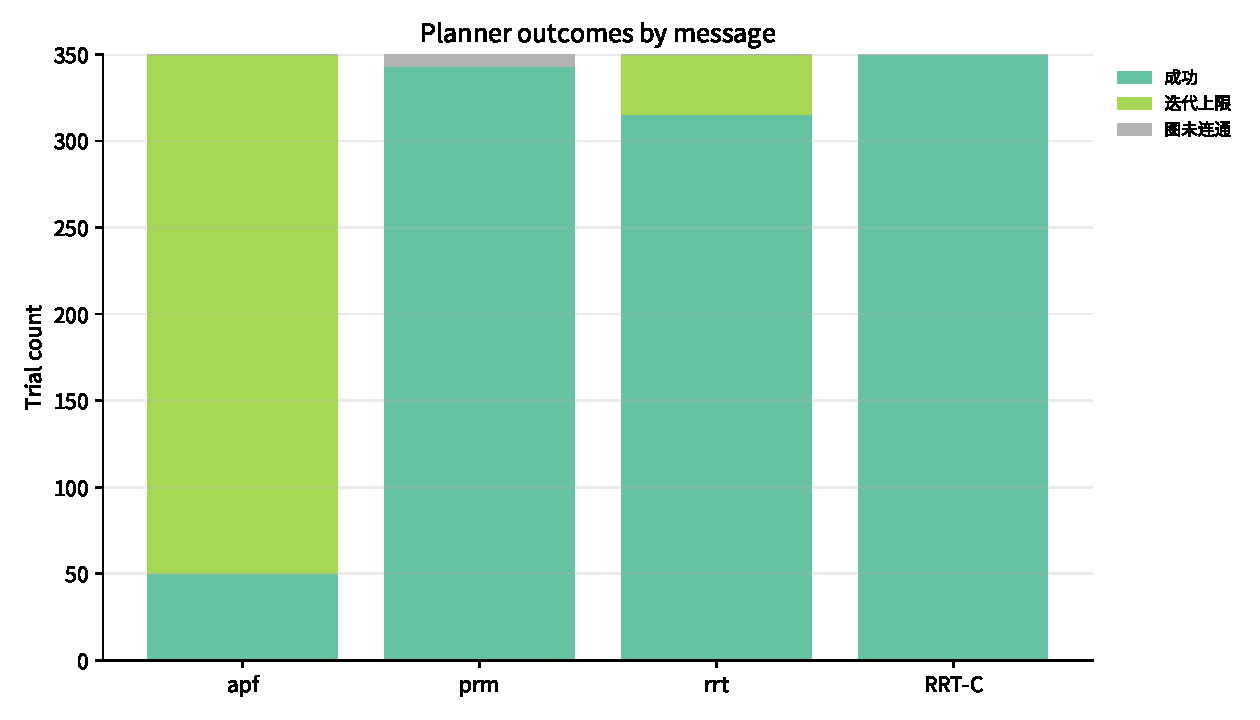
\includegraphics[width=0.86\linewidth,height=0.30\textheight,keepaspectratio]{generated/planner_failure_stacked.pdf}
  \caption{规划结果的失败原因统计。失败原因按论文级中文粗分类绘制，便于区分数值失败、碰撞失败和图搜索失败。}
  \label{fig:planner-failure-stacked}
\end{figure}

\begin{figure}[!htbp]
  \centering
  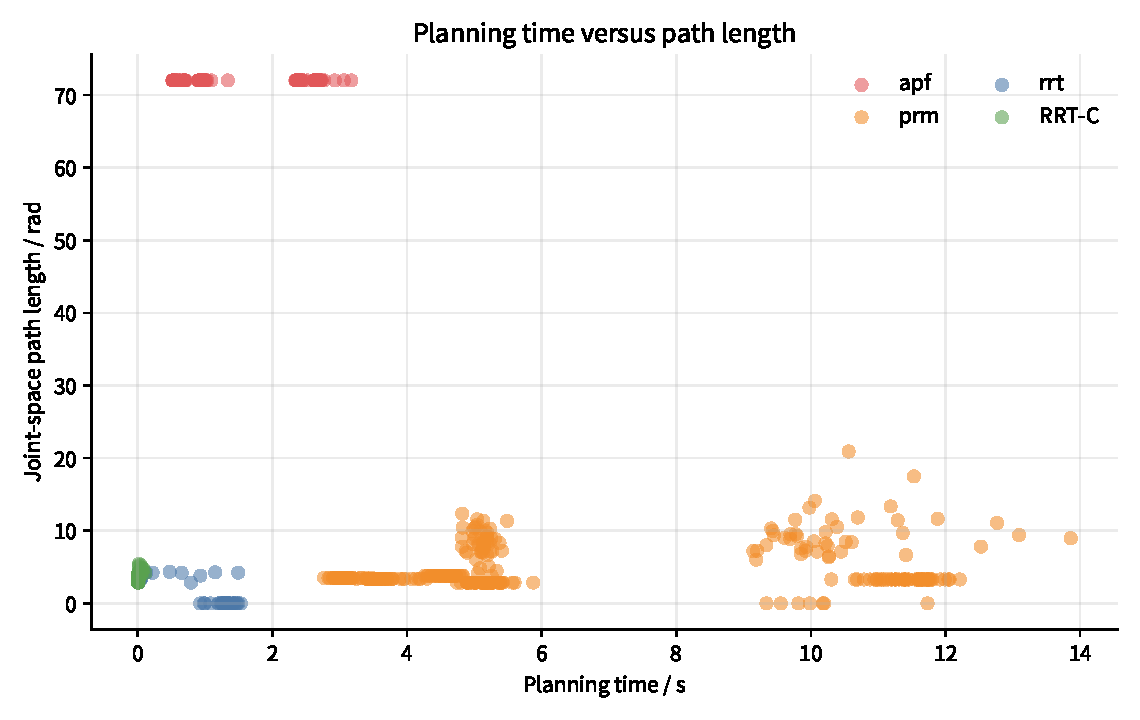
\includegraphics[width=0.86\linewidth,height=0.30\textheight,keepaspectratio]{generated/planner_time_length_scatter.pdf}
  \caption{规划耗时与路径长度关系。该图反映不同算法在效率和路径代价之间的差异。}
  \label{fig:planner-time-length-scatter}
\end{figure}

\begin{figure}[!htbp]
  \centering
  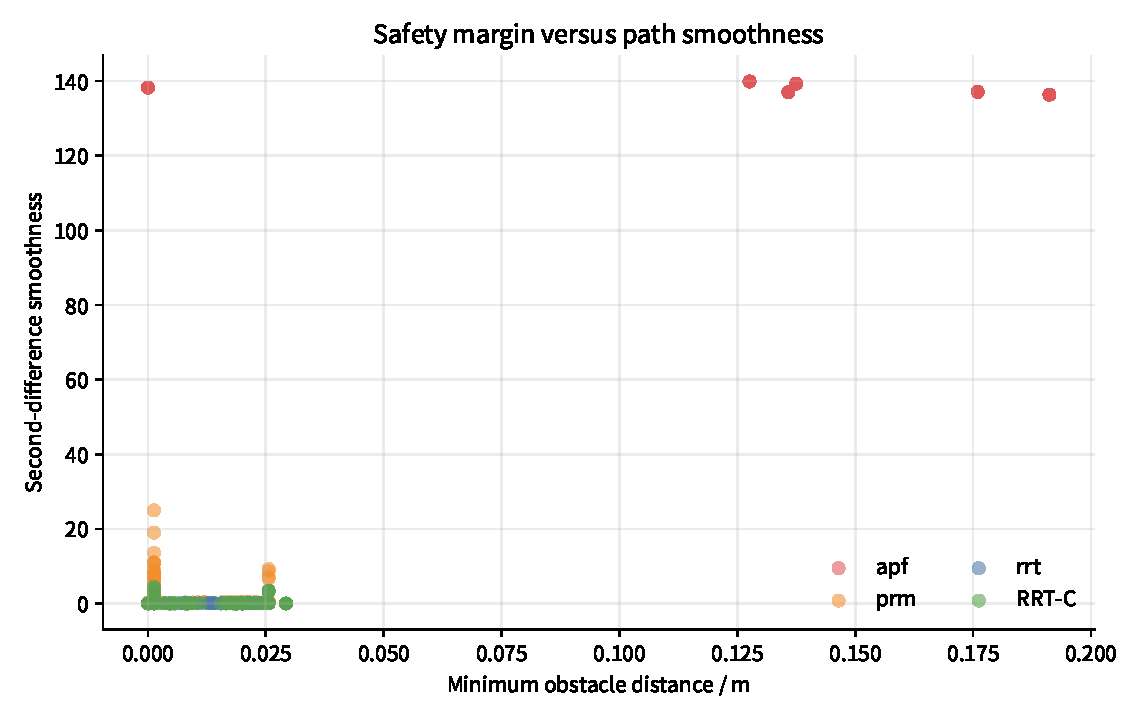
\includegraphics[width=0.86\linewidth,height=0.30\textheight,keepaspectratio]{generated/planner_safety_smoothness_scatter.pdf}
  \caption{安全距离与轨迹平滑度关系。该图用于观察更安全的路径是否伴随更高的轨迹弯曲或差分代价。}
  \label{fig:planner-safety-smoothness-scatter}
\end{figure}

失败原因在 CSV 中同时保存原始 message 和论文级粗分类。本文采用十类标签：成功、IK 未收敛、起点/目标无效、地面穿透、障碍碰撞、采样图未连通、局部极小值、迭代上限、后处理轨迹无效和其他。图 \ref{fig:planner-failure-stacked} 中的失败原因统计按中文粗分类绘制，以避免不同规划器内部消息过细导致图例不可读。其中“地面穿透”表示机器人任一碰撞几何体相对地面的最小距离小于 $-10^{-4}$ m；“后处理轨迹无效”表示原始规划路径成功，但 shortcut 或重采样后的路径在边插值复查中出现碰撞或穿地。

\section{实验平台与评价指标}

\subsection{实验流程}
实验平台由配置文件、仿真世界、IK 求解器、路径规划器、轨迹后处理、结果存储和绘图脚本组成。每个 trial 使用确定性种子生成，使随机采样算法可以复现。

整体数据流如图 \ref{fig:pipeline-blocks} 所示。根目录配置文件决定机器人模型、目标场景和算法参数；MuJoCo World 将这些配置实例化为可查询的仿真世界；IK 求解器先把目标位姿转换为目标关节构型；规划器在关节空间中搜索从起点到目标构型的可行路径；轨迹后处理负责 shortcut、重采样和边复查；最后由指标与绘图模块输出 CSV、summary 表和论文图。

\begin{figure}[!htbp]
  \centering
  \begin{tikzpicture}[node distance=0.75cm]
    \node[flowbox] (config) {配置文件\\run\_config.yaml};
    \node[flowbox, right=of config] (world) {MuJoCo World\\模型 + 障碍};
    \node[flowbox, right=of world] (ik) {IK 求解\\$\bm p_d,\bm s_d\rightarrow\bm q_g$};
    \node[flowbox, below=of ik] (planner) {规划器\\RRT / PRM / APF};
    \node[flowbox, left=of planner] (traj) {轨迹后处理\\shortcut + 重采样};
    \node[resultbox, left=of traj] (metrics) {指标与图表\\CSV / PDF / SVG};
    \draw[flowarrow] (config) -- (world);
    \draw[flowarrow] (world) -- (ik);
    \draw[flowarrow] (ik) -- (planner);
    \draw[flowarrow] (planner) -- (traj);
    \draw[flowarrow] (traj) -- (metrics);
  \end{tikzpicture}
  \caption{实验流程方块图。配置、仿真、IK、规划、轨迹后处理和指标导出构成完整闭环。}
  \label{fig:pipeline-blocks}
\end{figure}

\begin{equation}
  s_{i,j,t}
  =
  s_0+10000i+100j+t ,
  \label{eq:seed}
\end{equation}

其中 $i$ 表示场景编号，$j$ 表示算法编号，$t$ 表示 trial 编号。该公式避免不同场景和算法共享随机序列。
实验复现时，批量数据由 \path{run-experiments --config run_config.yaml --trials 50 --no-rerun} 生成，论文图片由 \path{export-plots --config run_config.yaml} 导出；这两个命令只作为实验流程的一部分说明，不再单独放入附录。

\begin{table}[!htbp]
  \centering
  \caption{实验参数设置}
  \label{tab:params}
  \begin{tabularx}{\textwidth}{p{4.0cm}X}
    \toprule
    参数 & 设置 \\
    \midrule
    IK 方法 & pinv、dls、lm、scipy\_baseline \\
    规划算法 & rrt、rrt\_connect、prm、apf \\
    场景数量 & 5 个固定基准场景 + 1 个主展示场景 \\
    重复次数 & 每场景每算法 50 次 \\
    边检测分辨率 & 0.06 rad \\
    轨迹重采样点数 & 80 \\
    全局随机种子 & 42 \\
    输出文件 & CSV、PDF/PNG 图表、Rerun 记录 \\
    \bottomrule
  \end{tabularx}
\end{table}

\subsection{程序结构与数据流}
代码实现按功能边界划分，而不是把所有逻辑写在一个脚本中。图 \ref{fig:code-architecture-blocks} 展示了核心模块之间的关系：配置模块负责读取 YAML 并解析场景，\texttt{MujocoWorld} 统一提供正运动学、姿态、碰撞和距离接口，IK 与规划器只依赖该统一接口；实验 runner 负责把不同算法组合成 trial，并把结果交给 metrics 和 plots 模块。

\begin{figure}[!htbp]
  \centering
  \begin{tikzpicture}[node distance=0.75cm and 0.55cm]
    \node[modulebox] (cfg) {config\\配置解析};
    \node[modulebox, right=of cfg] (world) {MujocoWorld\\仿真接口};
    \node[modulebox, right=of world] (ikmod) {ik.solvers\\目标构型};
    \node[modulebox, below=of world] (planner) {planners\\路径搜索};
    \node[modulebox, left=of planner] (smooth) {trajectory\\smoothing\\后处理};
    \node[modulebox, right=of planner] (runner) {experiments\\runner\\批量调度};
    \node[resultbox, below=of runner] (analysis) {metrics / plots\\统计与图表};
    \draw[flowarrow] (cfg) -- (world);
    \draw[flowarrow] (world) -- (ikmod);
    \draw[flowarrow] (ikmod) -- (planner);
    \draw[flowarrow] (world) -- (planner);
    \draw[flowarrow] (planner) -- (smooth);
    \draw[flowarrow] (smooth) -- (runner);
    \draw[flowarrow] (runner) -- (analysis);
  \end{tikzpicture}
  \caption{程序结构与数据流。统一仿真接口降低了 IK、规划器和指标模块之间的耦合。}
  \label{fig:code-architecture-blocks}
\end{figure}

命令行入口对应三类使用方式：\texttt{run-demo} 面向单组算法可视化，\texttt{run-all-combos} 遍历 16 组 IK/规划组合且只播放真实成功路径，\texttt{run-experiments} 与 \texttt{export-plots} 面向批量实验和论文图导出。这样的分工避免交互 demo 产生大量论文图片，也避免批量实验被可视化窗口阻塞。

\subsection{评价指标}
关节空间路径长度定义为
\begin{equation}
  L_q=\sum_{i=0}^{N-1}\norm{\bm q_{i+1}-\bm q_i}_2 .
  \label{eq:joint-length}
\end{equation}

任务空间路径长度定义为
\begin{equation}
  L_x=\sum_{i=0}^{N-1}\norm{f(\bm q_{i+1})-f(\bm q_i)}_2 .
  \label{eq:task-length}
\end{equation}

一阶差分近似关节速度增量：
\begin{equation}
  \Delta\bm q_i=\bm q_{i+1}-\bm q_i .
  \label{eq:first-diff}
\end{equation}

二阶差分近似加速度变化：
\begin{equation}
  \Delta^2\bm q_i=\bm q_{i+1}-2\bm q_i+\bm q_{i-1}.
  \label{eq:second-diff}
\end{equation}

平滑度指标取二阶差分范数和：
\begin{equation}
  S=\sum_{i=1}^{N-1}\norm{\Delta^2\bm q_i}_2 .
  \label{eq:smoothness}
\end{equation}

三阶差分用于衡量 jerk：
\begin{equation}
  \Delta^3\bm q_i
  =
  \bm q_{i+2}-3\bm q_{i+1}+3\bm q_i-\bm q_{i-1}.
  \label{eq:jerk}
\end{equation}

安全距离取路径上最小障碍距离：
\begin{equation}
  d_{\min}(\Pi)=\min_{\bm q_i\in\Pi}d(\bm q_i).
  \label{eq:min-distance}
\end{equation}

地面间隙单独记录，不并入障碍安全距离。设 $\mathcal G_r$ 为机器人碰撞几何体集合，$\mathcal G_f$ 为地面或 plane 几何体集合，则
\begin{equation}
  d_g(\bm q)
  =
  \min_{g_r\in\mathcal G_r,\ g_f\in\mathcal G_f}
  \operatorname{dist}(g_r(\bm q),g_f).
  \label{eq:ground-clearance}
\end{equation}

轨迹成功判定同时要求 IK、路径和执行约束满足：
\begin{equation}
  \begin{aligned}
  &\norm{f(\bm q_N)-\bm p_d}_2\leq \varepsilon_p,\\
  &\norm{\bm e_R(\bm q_N)}_2\leq \varepsilon_R\quad\text{若给定目标姿态},\\
  &d_{\min}(\bm q(\alpha))>0,\qquad
  d_g(\bm q(\alpha))\geq -10^{-4}\ \mathrm{m}.
  \end{aligned}
  \label{eq:success-criteria}
\end{equation}
其中 $\bm q(\alpha)$ 表示每条边上的离散插值点。地面穿透容差取 $-10^{-4}$ m，用于避免数值接触抖动造成误判；超过该容差的穿地轨迹被判为失败。

综合评分由成功率、耗时、路径长度、平滑度、安全距离、碰撞检测次数和终端误差归一化后平均得到：
\begin{equation}
  C=\frac{1}{K}\sum_{k=1}^{K}\hat m_k .
  \label{eq:composite}
\end{equation}

其中越小越好的指标先反向归一化，越大越好的指标直接归一化。各指标反映的物理含义不同：位置误差和姿态误差描述目标到达质量；路径长度和规划耗时描述效率；二阶、三阶差分描述轨迹执行平滑性；最小障碍距离和地面间隙描述安全裕度。若只报告成功率，可能把贴近障碍、加速度突变或穿地的路径误认为可执行；若只报告平滑度，又可能忽略目标误差和碰撞风险。因此本文采用多指标并列展示，并用综合评分作为辅助排序，而不是唯一评价依据。

\begin{figure}[!htbp]
  \centering
  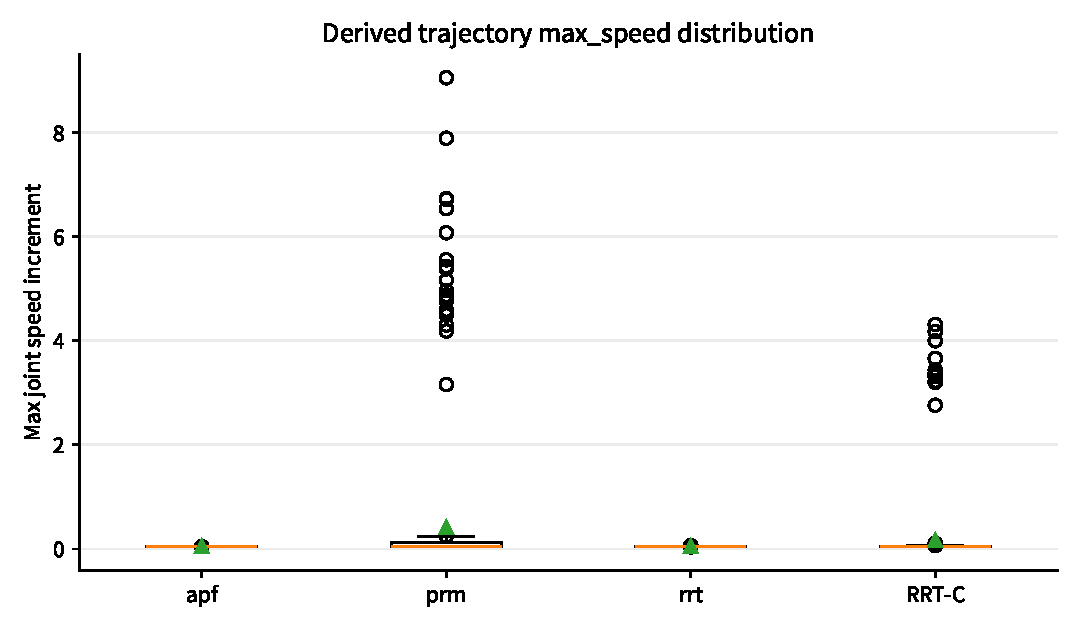
\includegraphics[width=0.86\linewidth,height=0.30\textheight,keepaspectratio]{generated/trajectory_derived_speed_boxplot.pdf}
  \caption{轨迹一阶差分速度增量分布。该图用于衡量不同规划器输出路径在相邻采样点之间的关节变化幅度。}
  \label{fig:trajectory-derived-speed}
\end{figure}

\begin{figure}[!htbp]
  \centering
  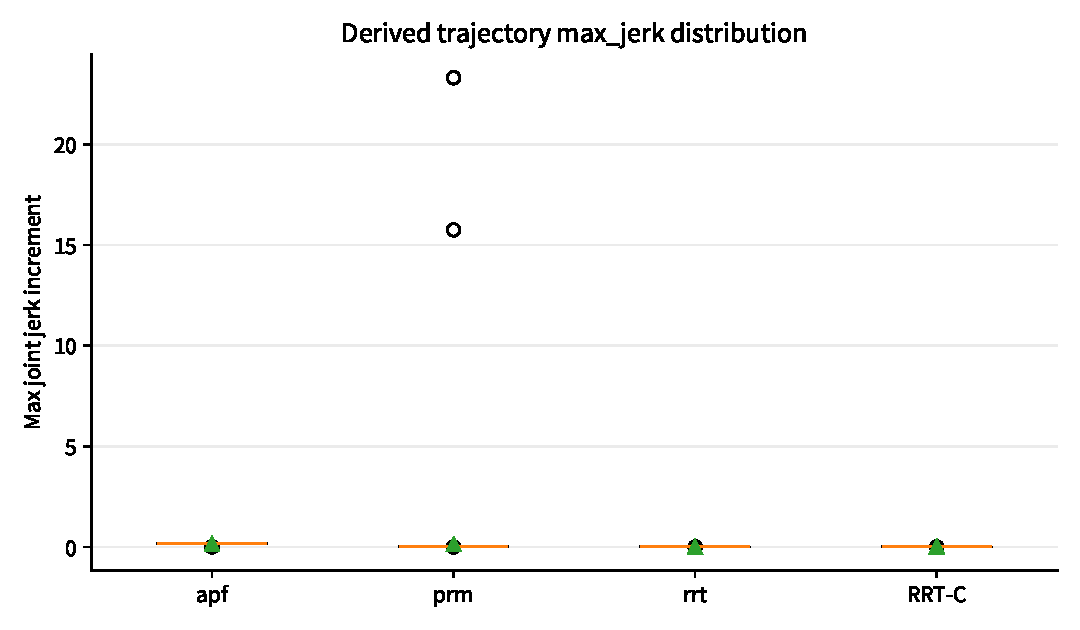
\includegraphics[width=0.86\linewidth,height=0.30\textheight,keepaspectratio]{generated/trajectory_derived_jerk_boxplot.pdf}
  \caption{轨迹三阶差分 jerk 增量分布。该图用于衡量轨迹高阶变化是否平滑，避免只用成功率评价可执行性。}
  \label{fig:trajectory-derived-jerk}
\end{figure}

\section{实验结果与讨论}

\subsection{多场景仿真画面证据}
为避免结果讨论只停留在抽象指标层面，本文首先给出七类代表性 MuJoCo 仿真画面。图 \ref{fig:mujoco-scene-no-obstacle}--图 \ref{fig:mujoco-scene-pass-through} 展示的是实际参与碰撞检测和距离计算的几何体，而不是后期绘制的示意图。因此，后文的成功率、安全距离、地面间隙和失败原因统计都可以回溯到这些具体空间约束。

\begin{figure}[!htbp]
  \centering
  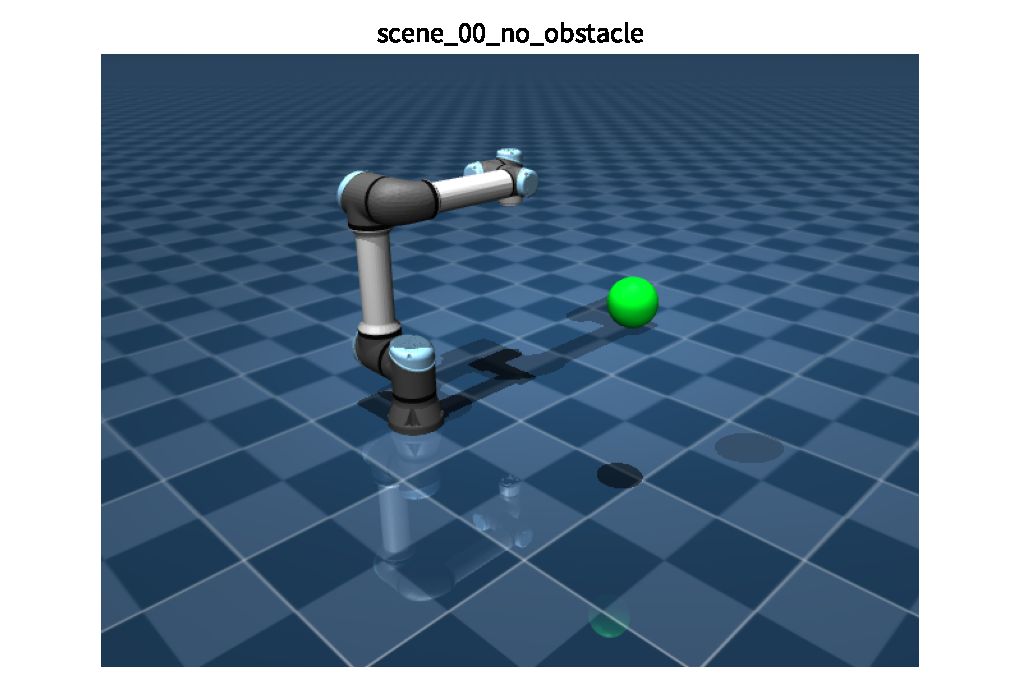
\includegraphics[width=0.78\linewidth,height=0.22\textheight,keepaspectratio]{generated/mujoco_scene_scene_00_no_obstacle.pdf}
  \caption{无障碍 MuJoCo 场景。该场景用于验证 IK 和规划器在没有外部碰撞约束时的基础可达性。}
  \label{fig:mujoco-scene-no-obstacle}
\end{figure}

\begin{figure}[!htbp]
  \centering
  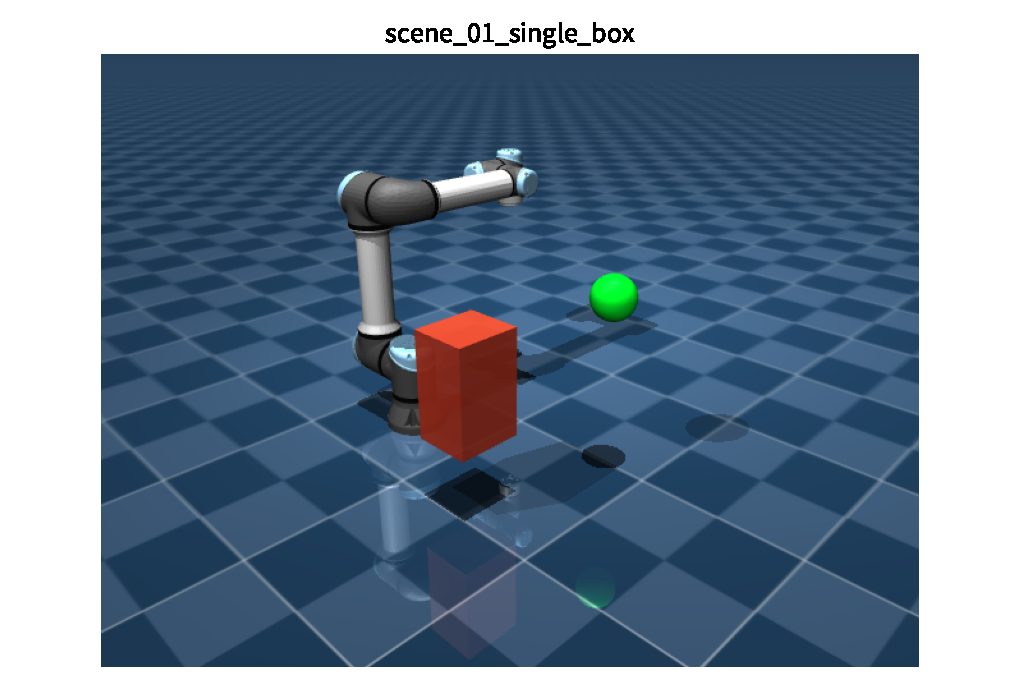
\includegraphics[width=0.78\linewidth,height=0.22\textheight,keepaspectratio]{generated/mujoco_scene_scene_01_single_box.pdf}
  \caption{单障碍 MuJoCo 场景。单个 box 与末端直线路径产生冲突，用于观察绕障和安全距离指标是否有效。}
  \label{fig:mujoco-scene-single-box}
\end{figure}

\begin{figure}[!htbp]
  \centering
  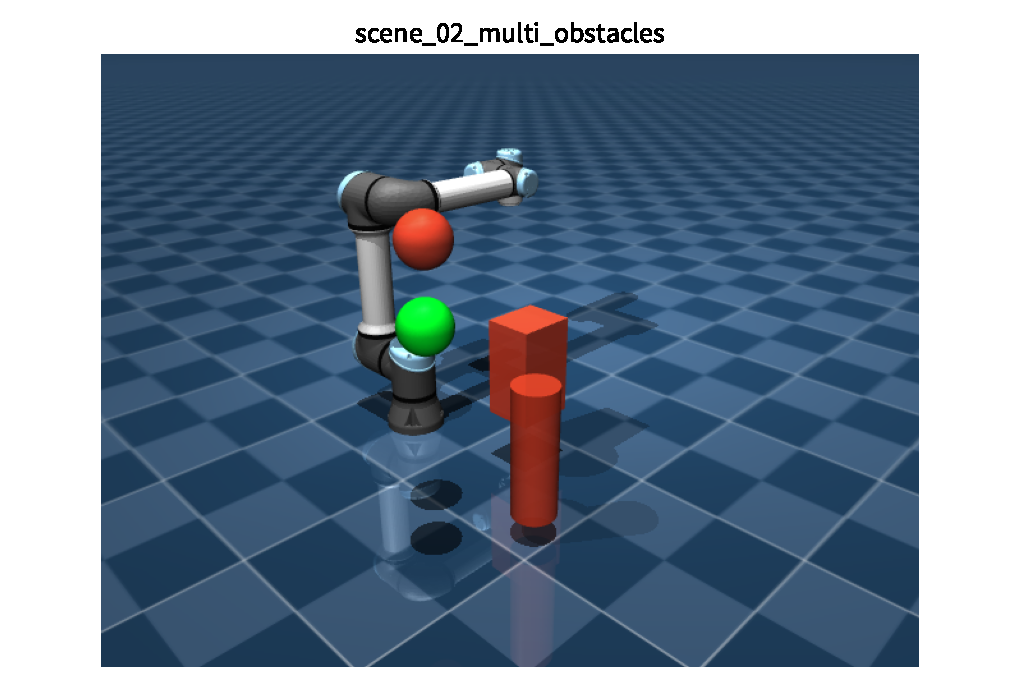
\includegraphics[width=0.78\linewidth,height=0.22\textheight,keepaspectratio]{generated/mujoco_scene_scene_02_multi_obstacles.pdf}
  \caption{多障碍 MuJoCo 场景。多个几何体同时压缩可行空间，用于检验随机采样和路线图连通性。}
  \label{fig:mujoco-scene-multi-obstacles}
\end{figure}

\begin{figure}[!htbp]
  \centering
  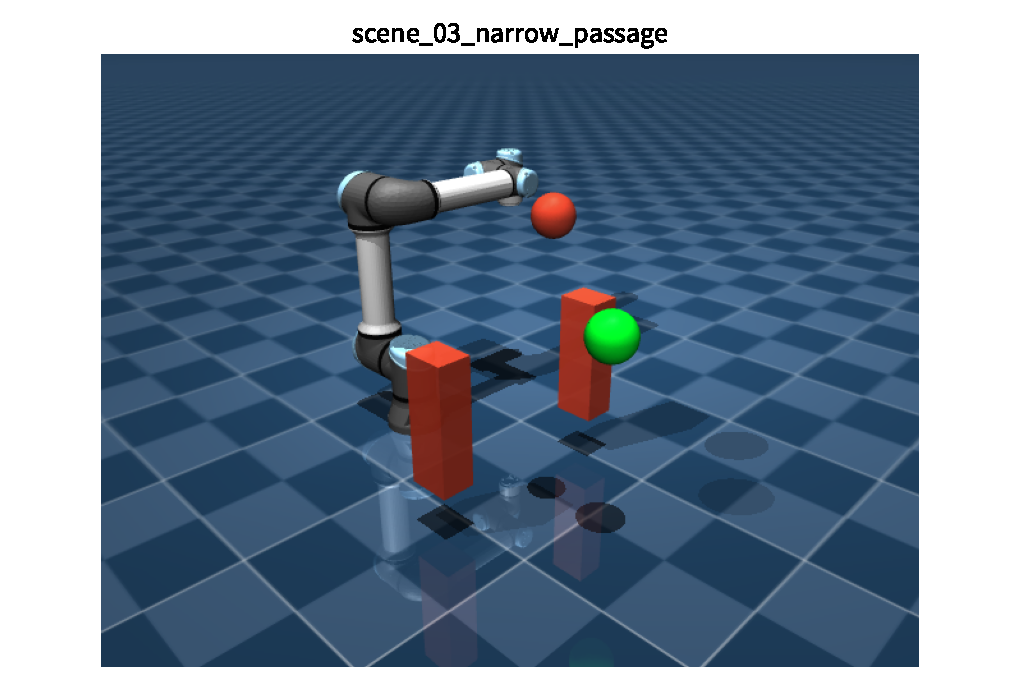
\includegraphics[width=0.78\linewidth,height=0.22\textheight,keepaspectratio]{generated/mujoco_scene_scene_03_narrow_passage.pdf}
  \caption{窄通道 MuJoCo 场景。左右墙体和顶部障碍形成局部通道，用于检验边插值碰撞检测和双向搜索优势。}
  \label{fig:mujoco-scene-narrow-passage}
\end{figure}

\begin{figure}[!htbp]
  \centering
  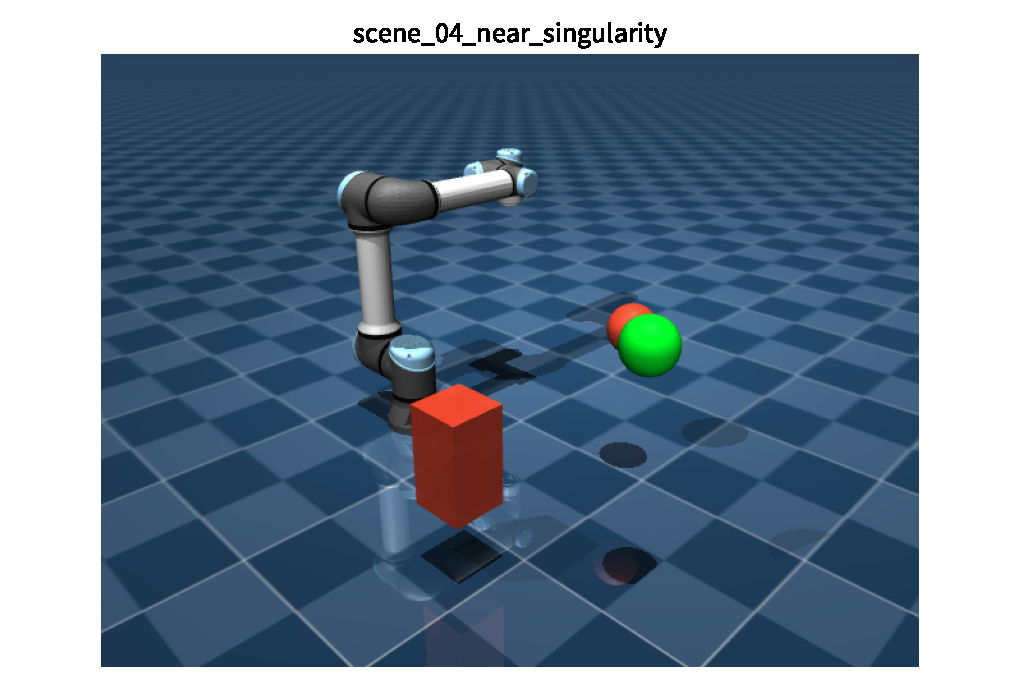
\includegraphics[width=0.78\linewidth,height=0.22\textheight,keepaspectratio]{generated/mujoco_scene_scene_04_near_singularity.pdf}
  \caption{近奇异 MuJoCo 场景。目标位置使机械臂更接近伸展位形，用于联系条件数、误差放大和关节增量。}
  \label{fig:mujoco-scene-near-singularity}
\end{figure}

\begin{figure}[!htbp]
  \centering
  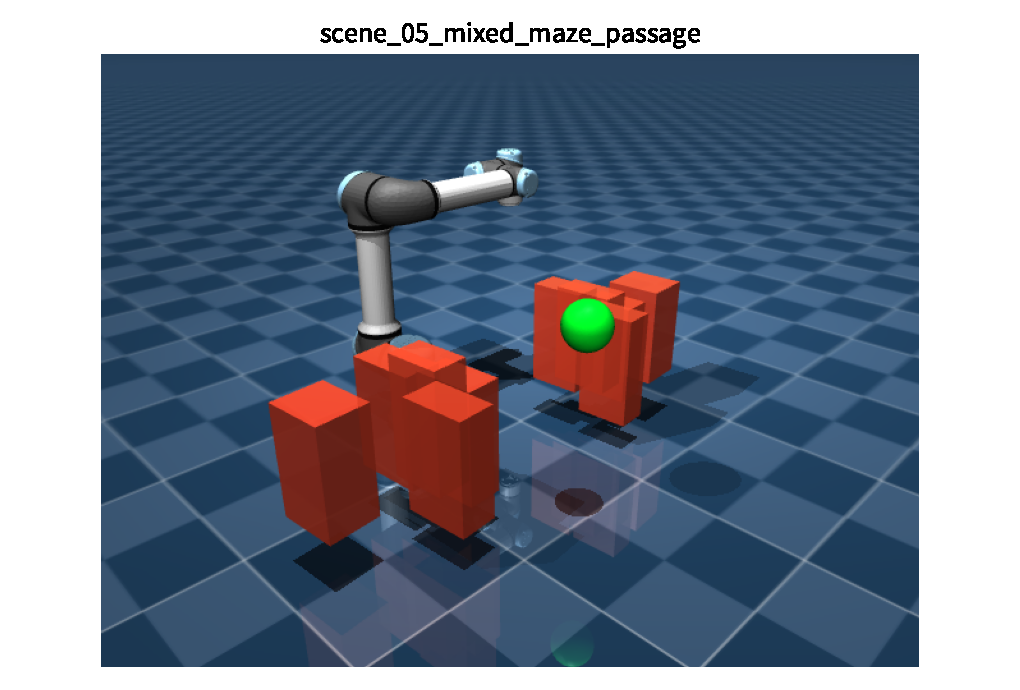
\includegraphics[width=0.78\linewidth,height=0.22\textheight,keepaspectratio]{generated/mujoco_scene_scene_05_mixed_maze_passage.pdf}
  \caption{混合迷宫通道 MuJoCo 场景。多组门洞和偏置障碍形成中等难度通道，是窄通道到小框插入任务之间的过渡案例。}
  \label{fig:mujoco-scene-mixed-maze}
\end{figure}

\begin{figure}[!htbp]
  \centering
  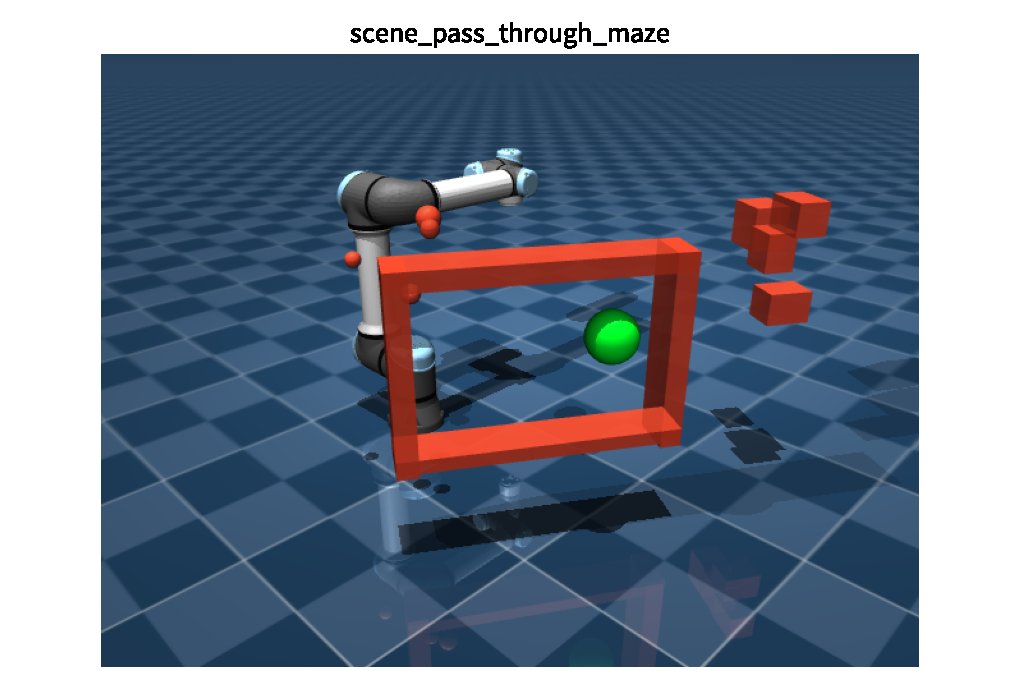
\includegraphics[width=0.78\linewidth,height=0.22\textheight,keepaspectratio]{generated/mujoco_scene_scene_pass_through_maze.pdf}
  \caption{小框插入 MuJoCo 场景。完整 UR5e 模型、姿态目标、小框和悬浮障碍叠加，用于综合验证避障规划可执行性。}
  \label{fig:mujoco-scene-pass-through}
\end{figure}

\subsection{多场景统计可信度说明}
本文的统计结果由多场景、固定随机种子和重复 trial 共同支撑。每个场景对应一个确定的 MuJoCo 几何布局；每个算法组合在该布局中使用可复现的 trial seed；每次 trial 的 IK 结果、规划结果、轨迹采样点和失败快照分别写入 CSV。这样设计的目的，是让论文中的每张图都能追溯到三类证据：场景图说明空间约束，过程曲线说明机器人如何运动，汇总表说明多次试验下的统计稳定性。

实验数据不是只保存最终成功或失败，而是同时保存末端位置、姿态四元数、累计任务空间长度、障碍距离、地面间隙以及关节速度、加速度和 jerk 范数。换言之，若某条轨迹虽然到达目标但在过程中贴近障碍、接近地面或出现高阶差分突变，这些现象都会反映在过程图中，而不会被单一成功率掩盖。

\subsection{IK 结果分析}
从图 \ref{fig:ik-error-boxplot} 和图 \ref{fig:ik-time-boxplot} 可见，SciPy 最小二乘基线的末端误差最低，中位误差达到 $10^{-8}$ m 量级，但中位求解时间约为 $0.0042$ s。Jacobian 伪逆、DLS 和 LM 的误差在毫米级到厘米级之间，中位求解时间通常小于 $0.0005$ s。若实验目标是生成高精度目标构型，SciPy 基线更适合作为离线参考；若目标是实时控制中的快速修正，阻尼 Jacobian 方法更具工程性价比。

近奇异场景的条件数明显升高。以 scene\_04\_near\_singularity 为例，多个方法的条件数 $p90$ 接近或超过 7，而无障碍场景约为 3.5。图 \ref{fig:ik-condition-heatmap} 和图 \ref{fig:ik-condition-error-scatter} 与式 \eqref{eq:condition} 一致：当最小奇异值变小，线性化子问题更敏感。DLS 和 LM 通过阻尼项降低了关节增量放大的风险，因此在报告中不只看最终误差，也同时报告条件数和耗时。

\begin{table}[!htbp]
  \centering
  \caption{IK 方法总体统计摘要}
  \label{tab:ik-summary-short}
  \small
  \begin{tabularx}{\textwidth}{lcccc}
    \toprule
    方法 & 成功率 & \makecell{误差中位数\\均值 / m} & \makecell{耗时中位数\\均值 / s} & \makecell{条件数\\$p90$ 均值} \\
    \midrule
    pinv & 1.00 & 0.006334 & 0.000400 & 4.091 \\
    dls & 1.00 & 0.007198 & 0.000271 & 4.125 \\
    lm & 1.00 & 0.006247 & 0.000266 & 4.112 \\
    scipy\_baseline & 1.00 & $5.35\times10^{-9}$ & 0.004202 & 4.258 \\
    \bottomrule
  \end{tabularx}
\end{table}

\subsection{算法适用性与优劣比较}
为了避免只按单一数值排名判断算法，本节把理论性质、实验表现和适用场景放在同一张表中比较。表 \ref{tab:ik-tradeoffs} 说明，IK 方法的核心取舍在于精度、速度和近奇异稳定性：伪逆法形式最直接，但对条件数敏感；DLS 和 LM 通过阻尼项牺牲少量收敛速度换取稳定性；SciPy 基线精度最高，适合作为离线参考而不是每个控制周期内的最轻量方案。

\begin{table}[!htbp]
  \centering
  \caption{IK 算法优劣与适用场景比较}
  \label{tab:ik-tradeoffs}
  \small
  \begin{tabularx}{\textwidth}{p{2.4cm}p{3.0cm}p{3.2cm}p{2.8cm}X}
    \toprule
    方法 & 主要优点 & 主要不足 & 实验表现 & 适用场景 \\
    \midrule
    pinv & 公式简单，单步计算快，远离奇异位形时误差下降直接。 & 对小奇异值敏感，可能放大关节增量。 & 速度快，误差为毫米到厘米级。 & 快速原型、远离奇异区域的在线修正。 \\
    dls & 阻尼项抑制奇异放大，更新更平滑。 & 阻尼过大时收敛保守，需要调节参数。 & 速度最快或接近最快，稳定性优于 pinv。 & 实时控制、近奇异风险较高的任务。 \\
    lm & 在 Gauss--Newton 与梯度下降之间折中。 & 参数和停止条件影响收敛行为。 & 精度与 DLS 接近，耗时仍较低。 & 需要稳定收敛且保留较快速度的任务。 \\
    scipy\_baseline & 非线性最小二乘实现成熟，终端误差最低。 & 耗时约高一个数量级，不利于高频闭环。 & 误差达到 $10^{-8}$ m 量级。 & 离线标定、基准解生成、论文对照实验。 \\
    \bottomrule
  \end{tabularx}
\end{table}

表 \ref{tab:planner-tradeoffs} 说明，规划算法的优劣取决于查询方式和环境结构。RRT 适合单次查询，但随机性使其在密集障碍中存在失败概率；RRT-Connect 通过双向连接提高了窄通道和远目标任务中的稳定性；PRM 构图成本较高，但如果同一环境中要反复查询多个起终点，它的路线图可以复用；APF 计算轻量、路径直观，却最容易陷入局部极小值，因此更适合作为轻量基线或局部修正方法。

\begin{table}[!htbp]
  \centering
  \caption{避障规划算法优劣与适用场景比较}
  \label{tab:planner-tradeoffs}
  \small
  \begin{tabularx}{\textwidth}{p{2.3cm}p{3.0cm}p{3.2cm}p{2.8cm}X}
    \toprule
    算法 & 主要优点 & 主要不足 & 实验表现 & 适用场景 \\
    \midrule
    RRT & 实现简单，单次查询开销低，能处理高维空间。 & 单树探索效率受随机采样影响，窄通道中可能耗尽迭代。 & 多障碍场景存在随机失败。 & 快速单次规划、障碍较稀疏任务。 \\
    RRT-Connect & 双向树加快起终点连接，成功率和耗时更稳定。 & 路径仍需后处理平滑，极窄通道仍依赖采样。 & 当前实验综合评分最高。 & 在线避障展示、单次查询和较复杂障碍环境。 \\
    PRM & 可复用路线图，适合多查询，成功率稳定。 & 前期构图和碰撞检测成本高。 & 成功率高但碰撞检测次数最多。 & 固定环境下多起终点查询。 \\
    APF & 计算轻量，路径生成连续，易解释。 & 缺少全局搜索，易陷入局部极小值。 & 单障碍、多障碍和窄通道中失败明显。 & 轻量基线、局部避障修正或与全局规划结合。 \\
    \bottomrule
  \end{tabularx}
\end{table}

\subsection{规划结果分析}
路径规划结果显示，RRT-Connect 在五个场景中均达到 100\% 成功率，并且在多数场景中规划耗时最低。图 \ref{fig:planner-success-heatmap} 显示 RRT 在多障碍场景成功率为 0.84，说明单树搜索在复杂障碍分布下更容易耗尽迭代次数。PRM 成功率稳定，但构图阶段带来较高碰撞检测次数。APF 在无障碍和近奇异场景可以成功，却在单障碍、多障碍和窄通道场景中全部达到最大迭代次数，这与局部极小值分析一致。

\begin{table}[!htbp]
  \centering
  \caption{规划算法总体统计摘要}
  \label{tab:planner-summary-short}
  \small
  \begin{tabularx}{\textwidth}{lccccc}
    \toprule
    算法 & 成功率 & \makecell{耗时中位数\\均值 / s} & 综合评分 & \makecell{安全距离\\$p10$ / m} & \makecell{碰撞检测\\$p90$} \\
    \midrule
    apf & 0.400 & 0.1288 & 0.6328 & 0.0726 & 858.00 \\
    prm & 1.000 & 0.7625 & 0.6580 & 0.0422 & 39369.86 \\
    rrt & 0.968 & 0.0123 & 0.9357 & 0.0410 & 776.08 \\
    rrt\_connect & 1.000 & 0.0013 & 0.9425 & 0.0408 & 75.24 \\
    \bottomrule
  \end{tabularx}
\end{table}

综合评分并不是唯一结论，但它有助于把多指标比较压缩成可读结果。双向 RRT-Connect 的综合评分均值为 0.9425，略高于 RRT 的 0.9357；二者差距不大，但双向连接策略在成功率和碰撞检测次数上更稳健。PRM 的成功率高，却因构图成本而在综合评分中落后。APF 的安全距离 $p10$ 看似较高，是因为许多失败路径没有真正穿过狭窄区域，不能据此认为 APF 更安全。图 \ref{fig:planner-time-length-scatter} 和图 \ref{fig:planner-safety-smoothness-scatter} 进一步说明，耗时、路径长度、安全距离和平滑度之间没有单调一致的优劣关系，需要结合具体任务解释。

\subsection{多场景仿真结果讨论}
多场景设计的目的不是简单增加实验数量，而是让不同数值问题在可观察的 MuJoCo 空间中出现。无障碍场景见图 \ref{fig:mujoco-scene-no-obstacle}，其作用是验证 IK 与规划器在没有外部障碍时能否稳定到达目标；若该场景失败，说明问题主要来自 IK 收敛、关节限位或规划器参数，而不是避障。单障碍场景见图 \ref{fig:mujoco-scene-single-box}，其作用是在末端路径和障碍之间引入明确冲突，使最小安全距离不再只是形式指标。

多障碍场景见图 \ref{fig:mujoco-scene-multi-obstacles}。多个 box、sphere 和 cylinder 同时压缩可行空间，RRT 的随机探索更容易在有限迭代内找不到连接路径，PRM 则需要更多采样点和近邻边才能形成连通图。图 \ref{fig:trajectory-single-box} 和图 \ref{fig:trajectory-multi-obstacles} 对比可以看到，多障碍轨迹比单障碍轨迹更弯曲，这与表 \ref{tab:planner-summary-short} 中 PRM 碰撞检测次数较高、RRT 存在随机失败相互印证。

\begin{figure}[!htbp]
  \centering
  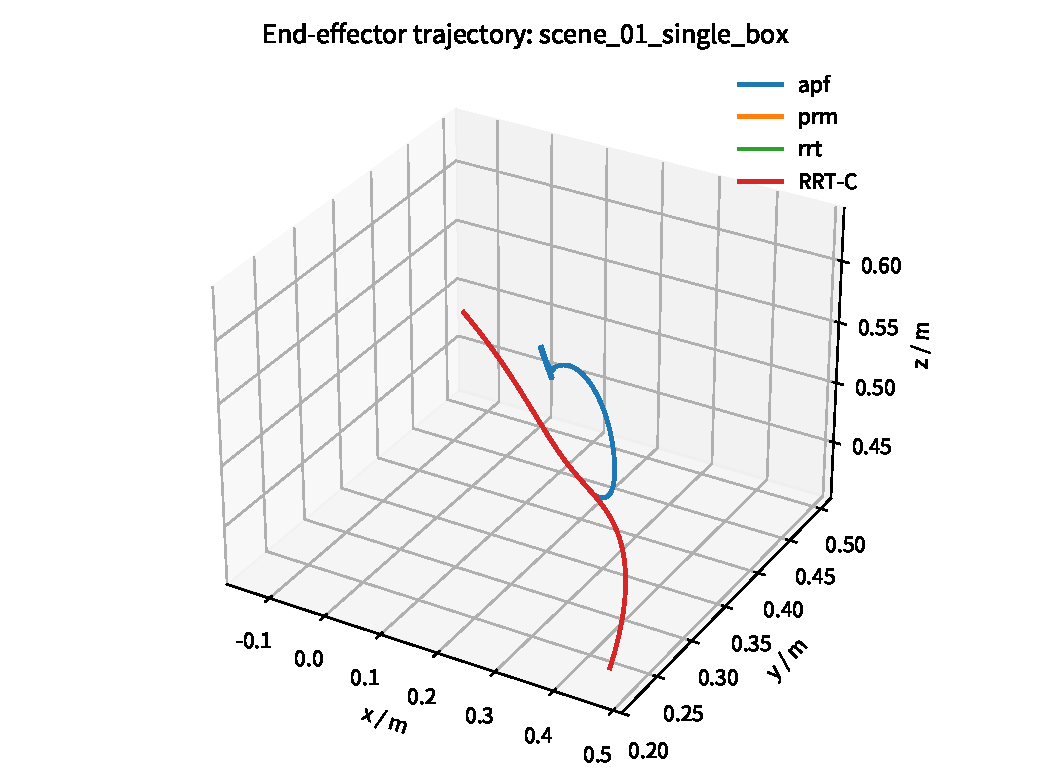
\includegraphics[width=0.82\linewidth,height=0.26\textheight,keepaspectratio]{generated/ee_trajectory_scene_01_single_box.pdf}
  \caption{单障碍场景的末端轨迹。轨迹绕过单个 box 后到达目标，用于说明安全距离指标的物理含义。}
  \label{fig:trajectory-single-box}
\end{figure}

\begin{figure}[!htbp]
  \centering
  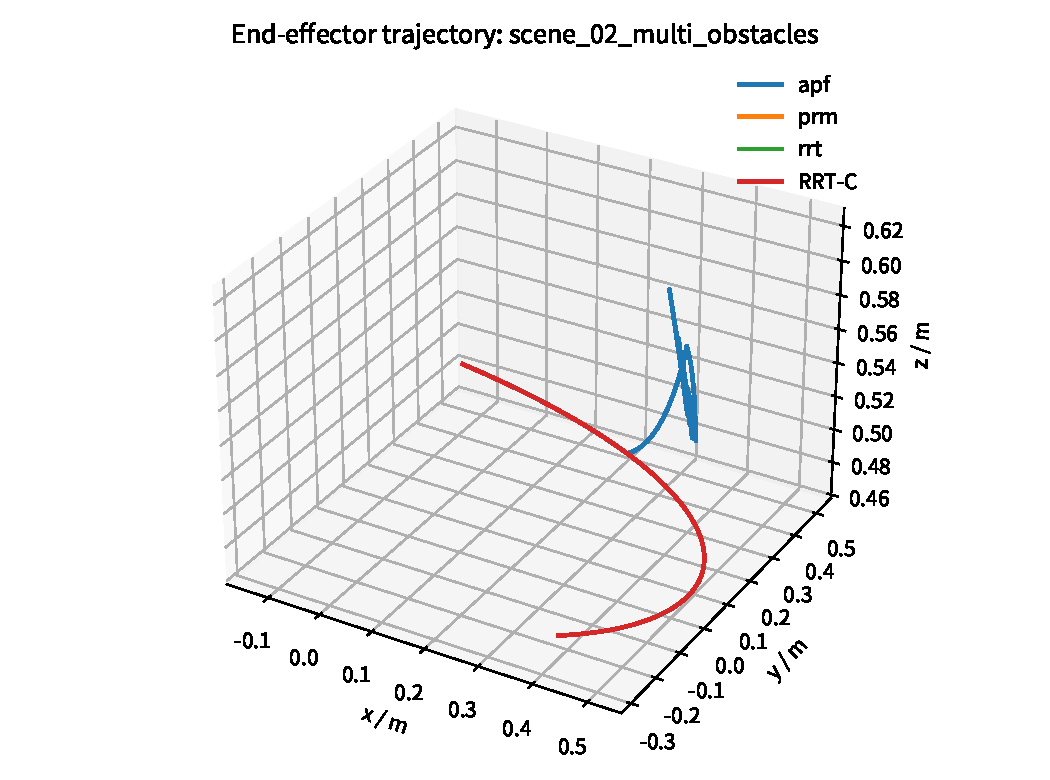
\includegraphics[width=0.82\linewidth,height=0.26\textheight,keepaspectratio]{generated/ee_trajectory_scene_02_multi_obstacles.pdf}
  \caption{多障碍场景的末端轨迹。障碍数量增加后，轨迹更依赖采样连通性和边插值检测。}
  \label{fig:trajectory-multi-obstacles}
\end{figure}

窄通道场景见图 \ref{fig:mujoco-scene-narrow-passage}，其难点不是目标远，而是可行边必须穿过较窄空间；这使边检测分辨率直接影响成功判定。RRT-Connect 的双向树能从起点和目标两端同时接近通道，因此比单树 RRT 更稳定。近奇异场景见图 \ref{fig:mujoco-scene-near-singularity}，其障碍不一定最复杂，但目标接近伸展位形，Jacobian 最小奇异值变小，关节增量更容易被放大。

混合迷宫通道见图 \ref{fig:mujoco-scene-mixed-maze}，它处于窄通道和小框插入之间：障碍不只是左右两面墙，而是沿路径方向形成若干门洞和偏置约束。该场景的价值在于检验算法是否只会从外围绕行，还是能在多组几何约束之间保持可行连接。小框插入场景见图 \ref{fig:mujoco-scene-pass-through}，作为综合案例叠加完整 UR5e 模型、姿态目标、地面约束和密集悬浮障碍，用于展示最终系统在更接近真实仿真的条件下仍能输出可解释轨迹。

\begin{figure}[!htbp]
  \centering
  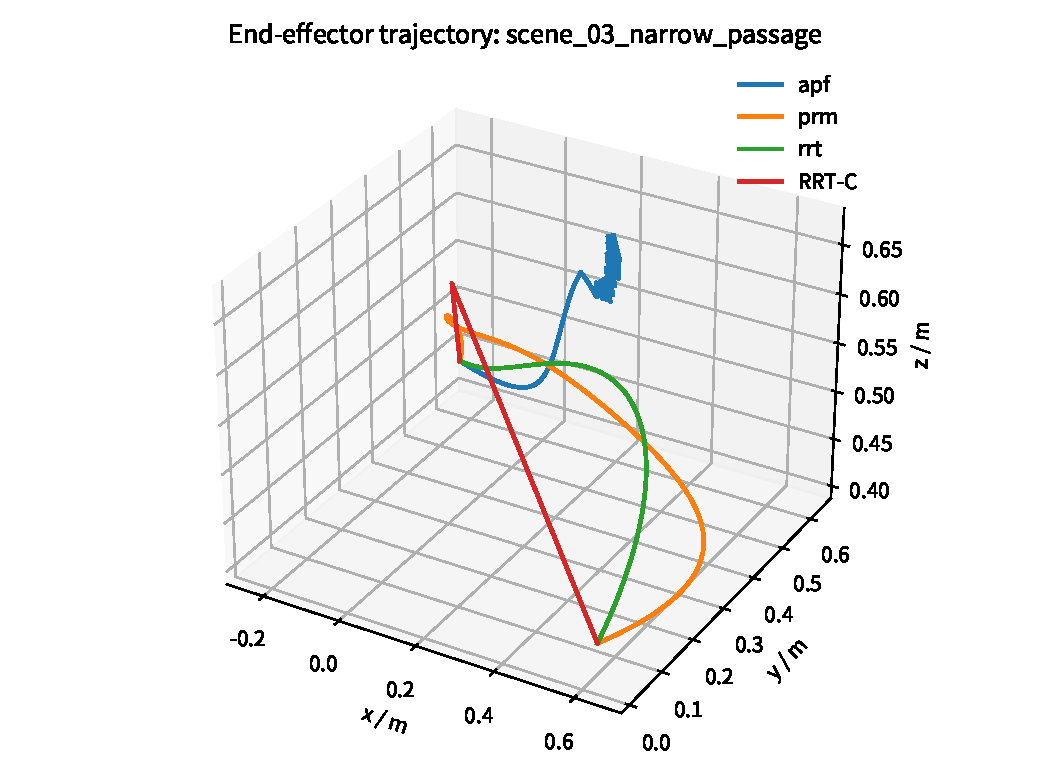
\includegraphics[width=0.82\linewidth,height=0.26\textheight,keepaspectratio]{generated/ee_trajectory_scene_03_narrow_passage.pdf}
  \caption{窄通道场景的末端轨迹。可行路径被局部通道约束，双向搜索更容易从两端逼近连接区域。}
  \label{fig:trajectory-narrow-passage-single}
\end{figure}

\begin{figure}[!htbp]
  \centering
  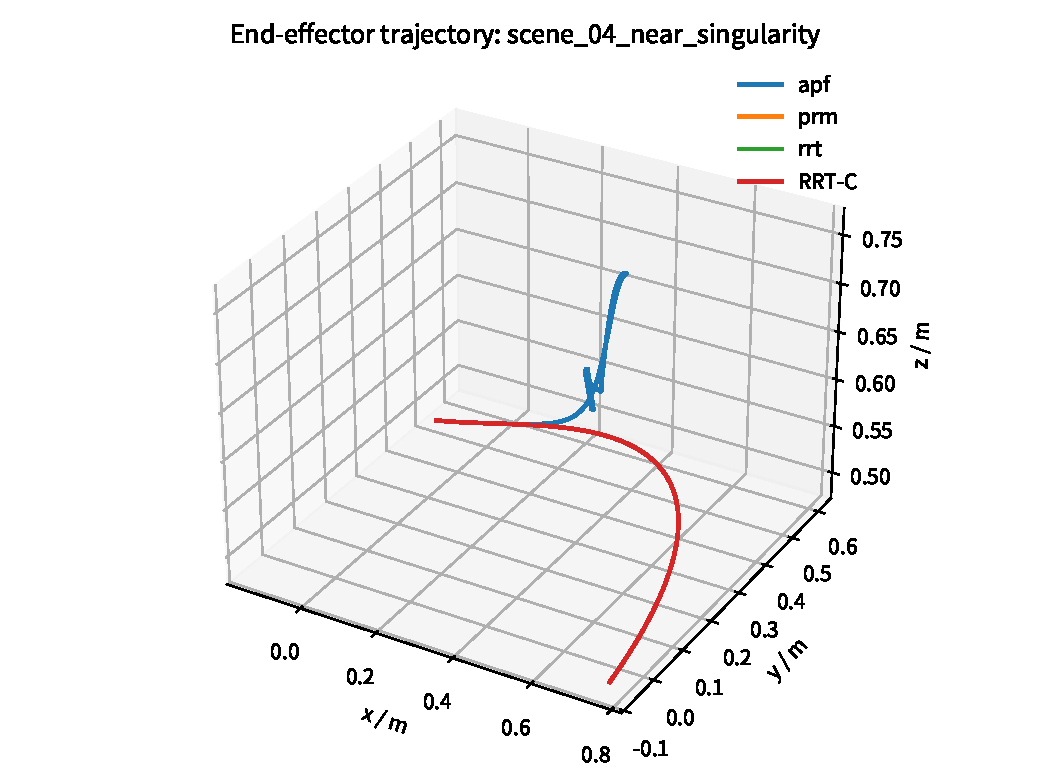
\includegraphics[width=0.82\linewidth,height=0.26\textheight,keepaspectratio]{generated/ee_trajectory_scene_04_near_singularity.pdf}
  \caption{近奇异场景的末端轨迹。该图配合条件数热力图，用于说明 IK 数值敏感性如何传递到规划目标构型。}
  \label{fig:trajectory-near-singularity-single}
\end{figure}

\begin{figure}[!htbp]
  \centering
  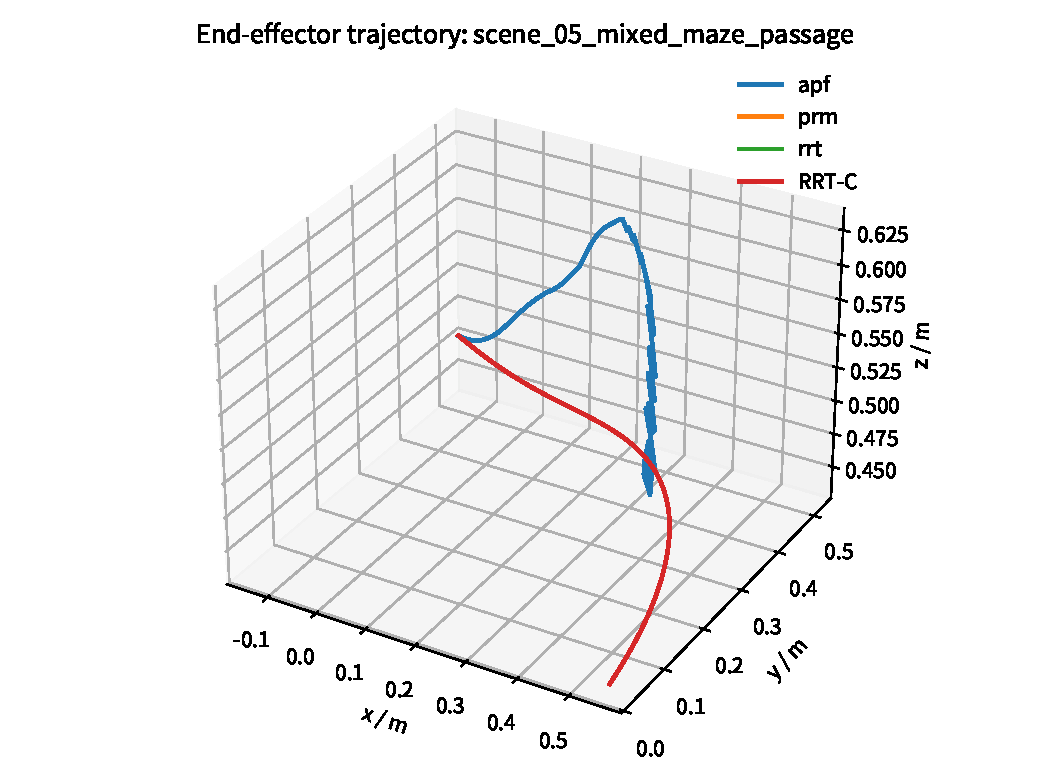
\includegraphics[width=0.82\linewidth,height=0.26\textheight,keepaspectratio]{generated/ee_trajectory_scene_05_mixed_maze_passage.pdf}
  \caption{混合迷宫通道场景的末端轨迹。该图展示多组门洞约束下的中等难度通道规划过程。}
  \label{fig:trajectory-mixed-maze-single}
\end{figure}

\begin{figure}[!htbp]
  \centering
  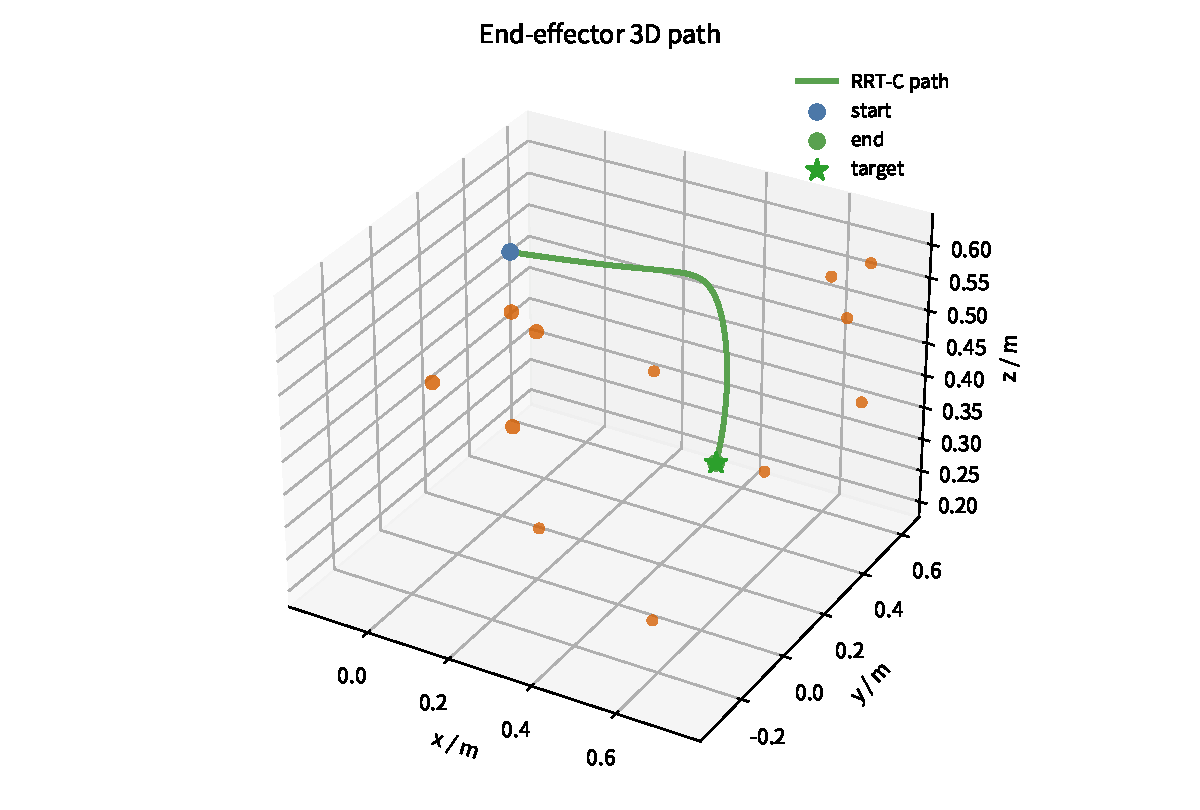
\includegraphics[width=0.82\linewidth,height=0.26\textheight,keepaspectratio]{generated/paper_ee_path_3d_large.pdf}
  \caption{小框插入场景的末端三维轨迹。该综合场景同时包含目标姿态、地面约束、悬浮障碍和插入式终点。}
  \label{fig:trajectory-pass-through-single}
\end{figure}

因此，多场景结果形成了由易到难的证据链：MuJoCo 场景图说明空间约束真实存在，末端轨迹图说明算法如何在这些约束中运动，CSV 指标和统计图则量化误差、安全距离、地面间隙和平滑性。主展示场景不是唯一依据，而是把前述多场景中出现的数值问题集中到一个更复杂的完整 UR5e 仿真案例中。

\subsection{轨迹可视化与运动学解释}
末端轨迹图展示了不同场景中路径绕障的空间形态。无障碍场景中各算法路径接近直接连接；多障碍和窄通道场景中，采样算法会绕开障碍形成更长但可行的关节空间路径。轨迹差分图进一步说明，路径是否可执行不能只看成功率，还要看速度、加速度和 jerk 是否平滑。

\begin{figure}[!htbp]
  \centering
  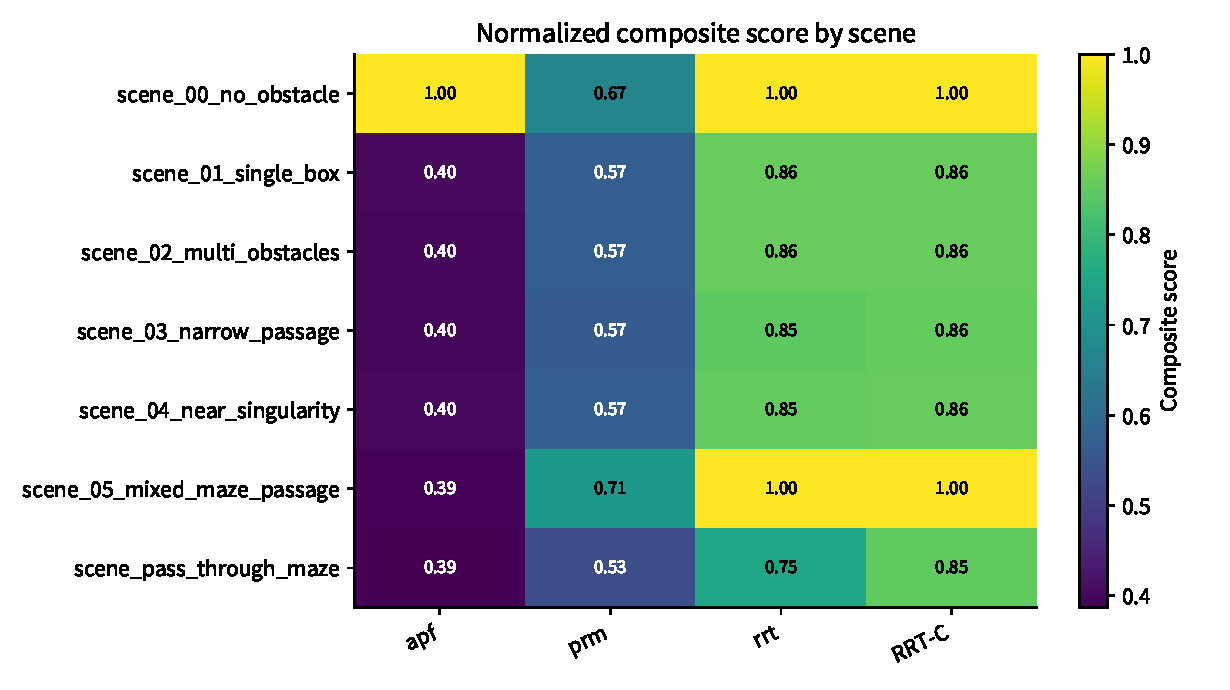
\includegraphics[width=0.86\linewidth,height=0.30\textheight,keepaspectratio]{generated/planner_composite_heatmap.pdf}
  \caption{规划器综合评分热力图。该图把成功率、耗时、路径长度、平滑度、安全距离、碰撞检测次数和终端误差压缩为辅助排序指标。}
  \label{fig:planner-composite-heatmap}
\end{figure}

\begin{figure}[!htbp]
  \centering
  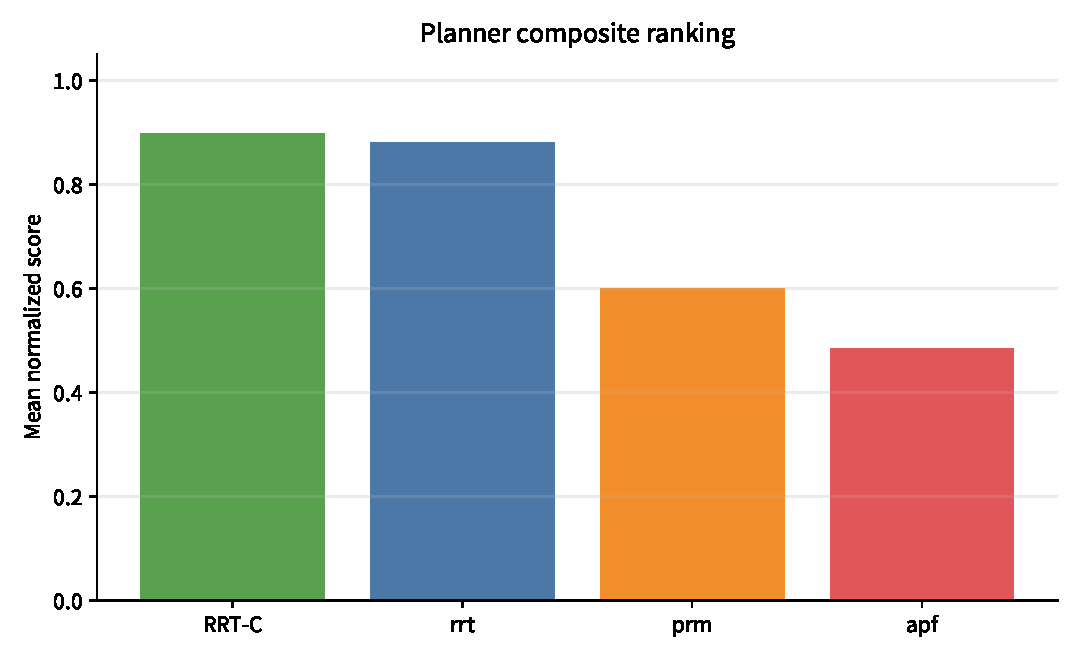
\includegraphics[width=0.86\linewidth,height=0.30\textheight,keepaspectratio]{generated/planner_composite_ranking.pdf}
  \caption{规划器综合排名。RRT-Connect 在成功率、耗时和碰撞检测次数之间取得较均衡表现。}
  \label{fig:planner-composite-ranking}
\end{figure}

\begin{figure}[!htbp]
  \centering
  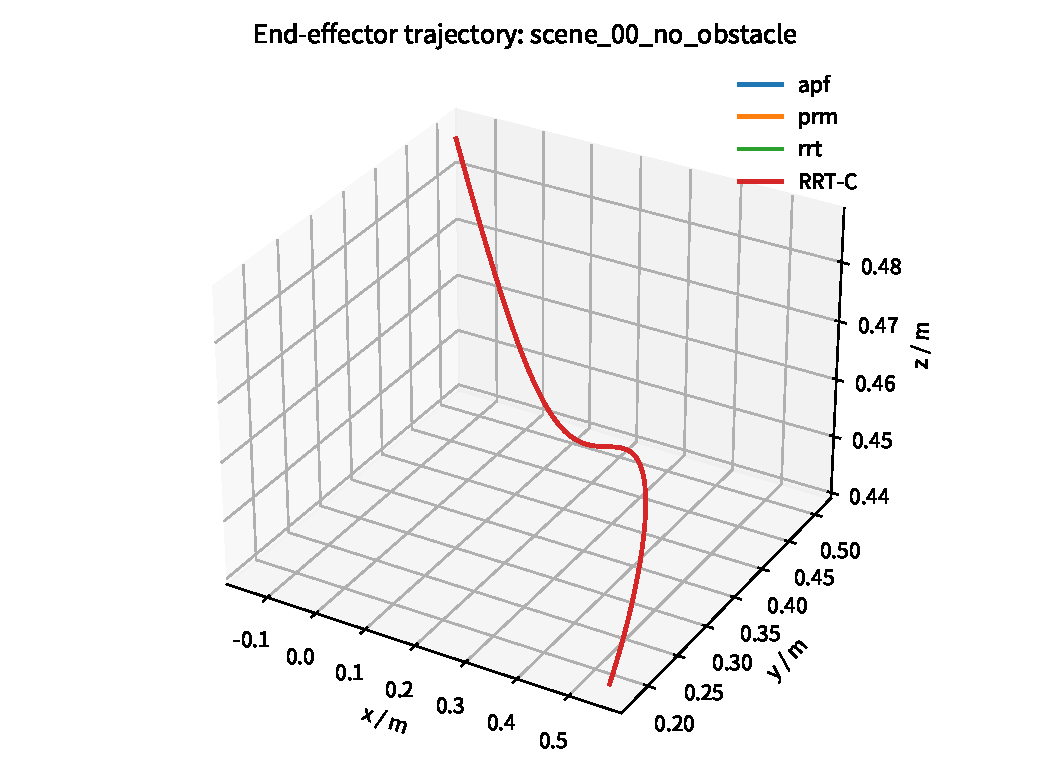
\includegraphics[width=0.86\linewidth,height=0.30\textheight,keepaspectratio]{generated/ee_trajectory_3d.pdf}
  \caption{无障碍场景下的末端三维轨迹。该图作为基线，用于说明无障碍时路径接近直接连接。}
  \label{fig:ee-trajectory-3d}
\end{figure}

\begin{figure}[!htbp]
  \centering
  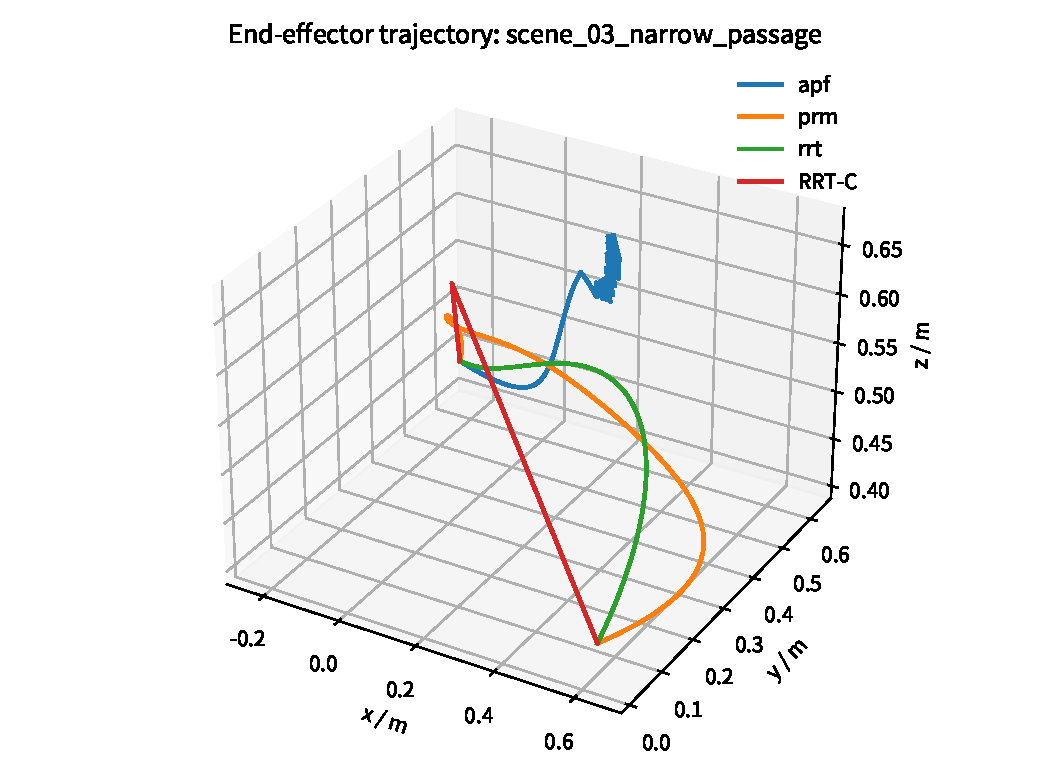
\includegraphics[width=0.86\linewidth,height=0.30\textheight,keepaspectratio]{generated/ee_trajectory_scene_03_narrow_passage.pdf}
  \caption{窄通道场景下的末端轨迹。采样式规划器需要绕开两侧墙体和顶部障碍，因此轨迹形态比无障碍场景更弯曲。}
  \label{fig:ee-trajectory-narrow}
\end{figure}

\subsection{过程数据与可执行性分析}
过程数据用于回答“轨迹在运动过程中是否可信”，而不是只回答“最终是否到达”。图 \ref{fig:paper-ee-position-x}--图 \ref{fig:paper-ee-position-z} 将末端三维位置拆开显示，可以观察轨迹是否存在突跳；图 \ref{fig:paper-cumulative-task-length} 显示累计任务空间路径长度，若曲线中段突然变陡，说明轨迹在该阶段发生较大空间绕行。

\begin{figure}[!htbp]
  \centering
  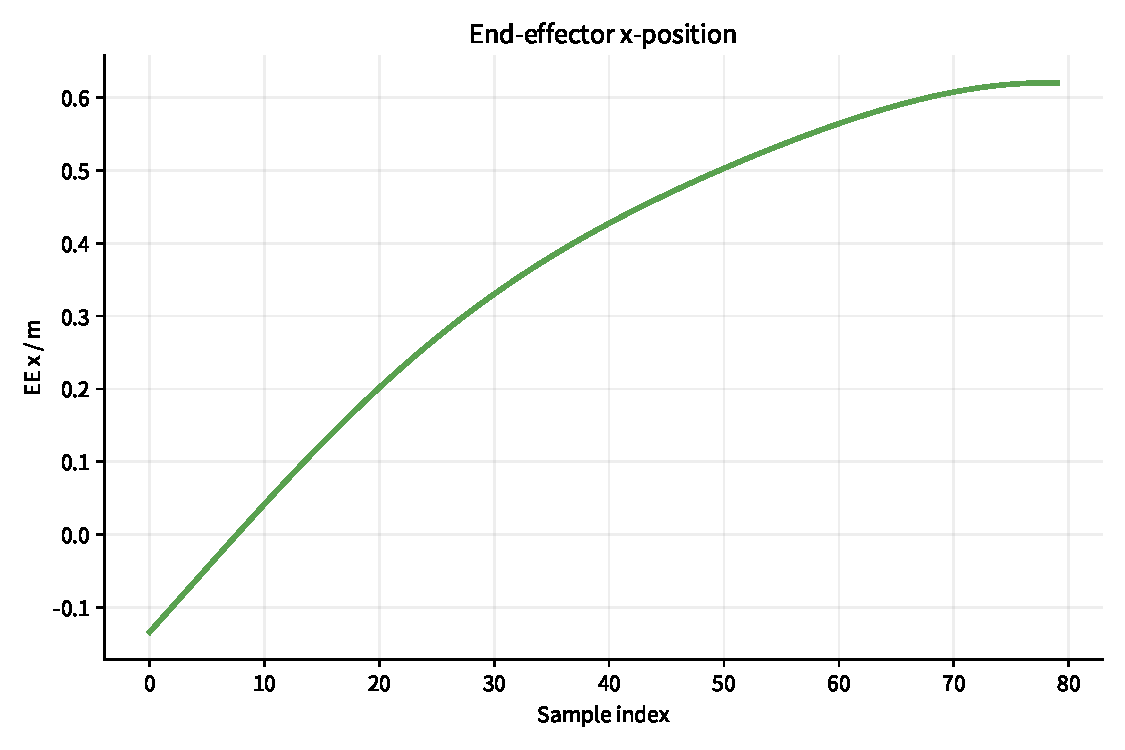
\includegraphics[width=0.82\linewidth,height=0.25\textheight,keepaspectratio]{generated/paper_ee_position_x.pdf}
  \caption{主展示轨迹的末端 $x$ 方向位置过程。单独显示坐标分量可以发现三维轨迹图中不易观察的单轴变化。}
  \label{fig:paper-ee-position-x}
\end{figure}

\begin{figure}[!htbp]
  \centering
  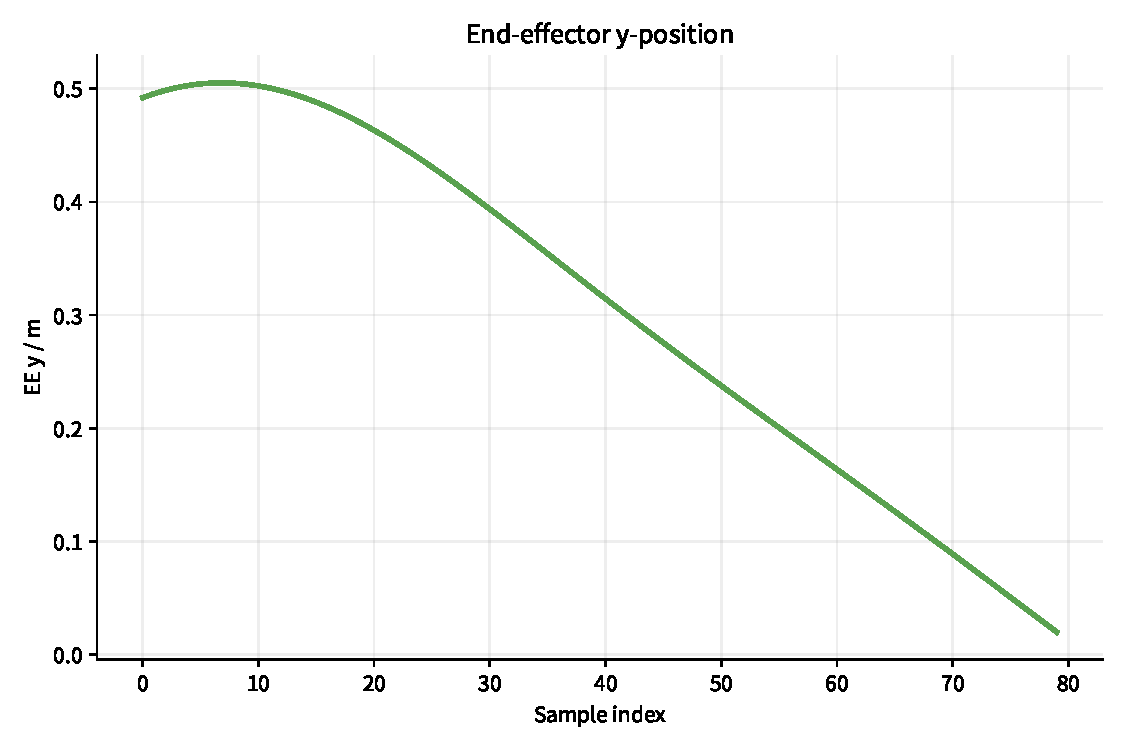
\includegraphics[width=0.82\linewidth,height=0.25\textheight,keepaspectratio]{generated/paper_ee_position_y.pdf}
  \caption{主展示轨迹的末端 $y$ 方向位置过程。该分量反映末端相对障碍通道中心线的横向偏移。}
  \label{fig:paper-ee-position-y}
\end{figure}

\begin{figure}[!htbp]
  \centering
  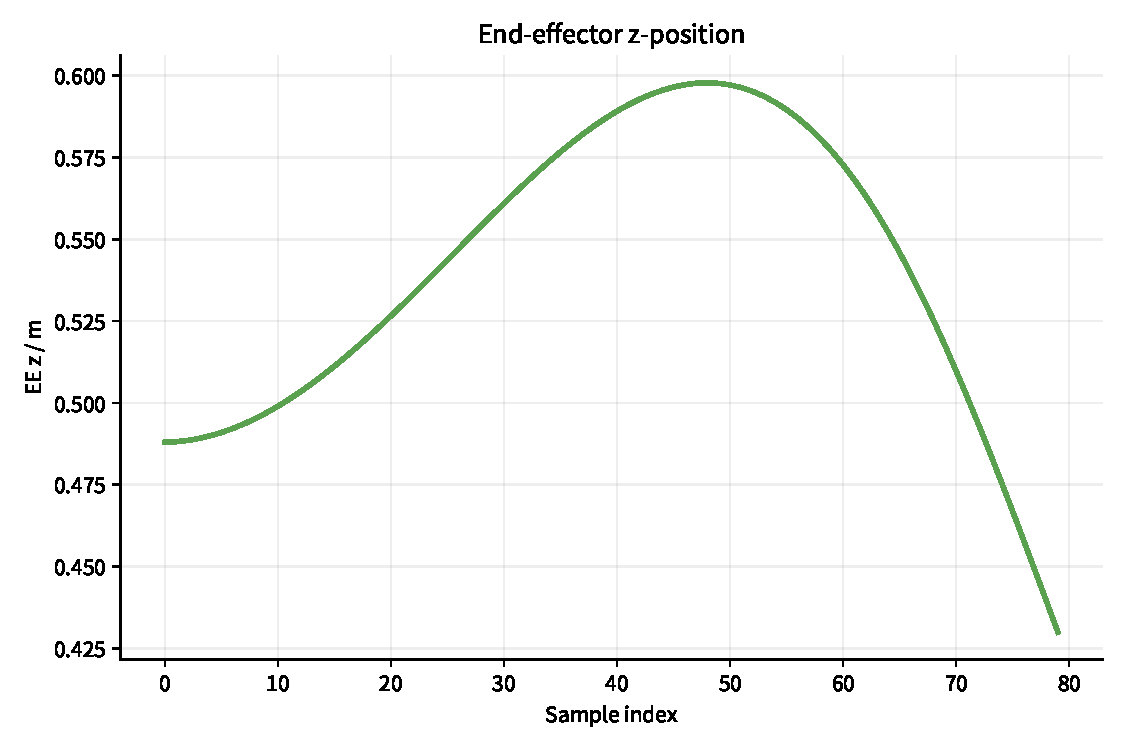
\includegraphics[width=0.82\linewidth,height=0.25\textheight,keepaspectratio]{generated/paper_ee_position_z.pdf}
  \caption{主展示轨迹的末端 $z$ 方向位置过程。该分量用于检查末端高度是否平稳，并辅助判断地面约束裕度。}
  \label{fig:paper-ee-position-z}
\end{figure}

\begin{figure}[!htbp]
  \centering
  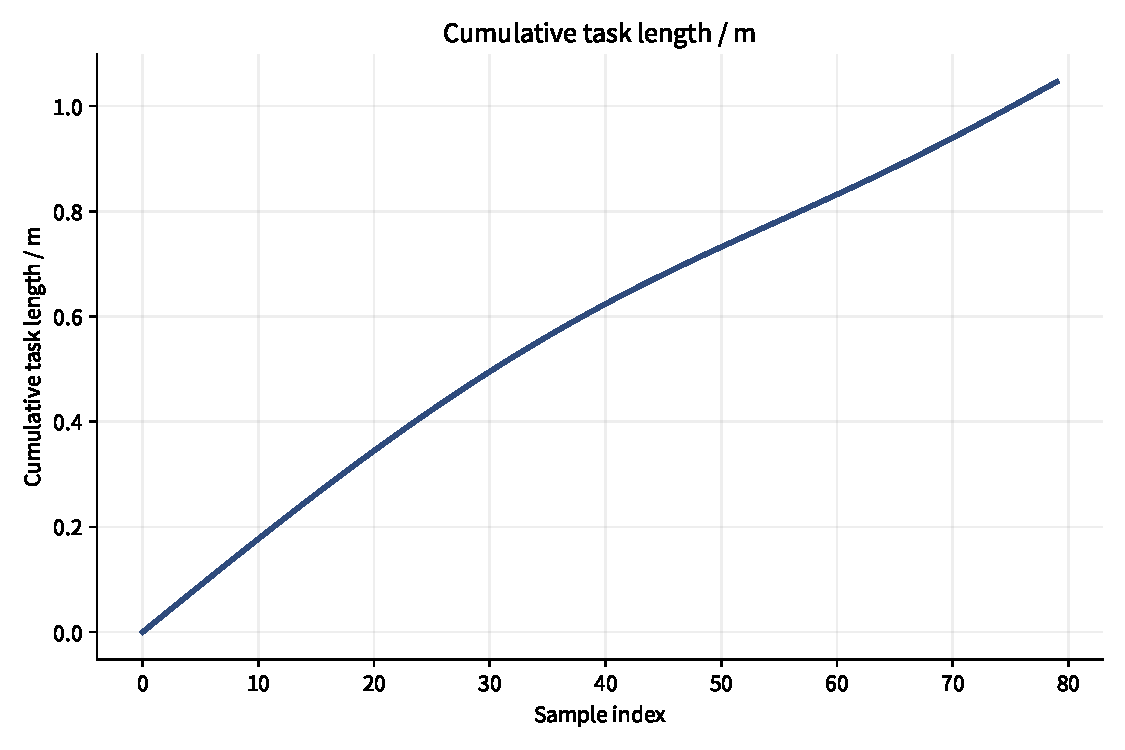
\includegraphics[width=0.82\linewidth,height=0.25\textheight,keepaspectratio]{generated/paper_cumulative_task_length.pdf}
  \caption{主展示轨迹的累计任务空间路径长度。曲线斜率越大，表示相邻采样点之间末端空间位移越大。}
  \label{fig:paper-cumulative-task-length}
\end{figure}

误差过程和安全过程直接对应成功判定。图 \ref{fig:paper-ee-position-error} 显示末端位置误差是否逐步接近目标；图 \ref{fig:paper-ee-orientation-error} 显示姿态约束是否同步收敛；图 \ref{fig:paper-min-obstacle-distance} 显示机械臂几何体到最近障碍的距离；图 \ref{fig:paper-min-ground-clearance} 则显示到地面 plane 的最小间隙。只有这些曲线同时处于合理范围，终点误差小的轨迹才具备物理可执行性。

\begin{figure}[!htbp]
  \centering
  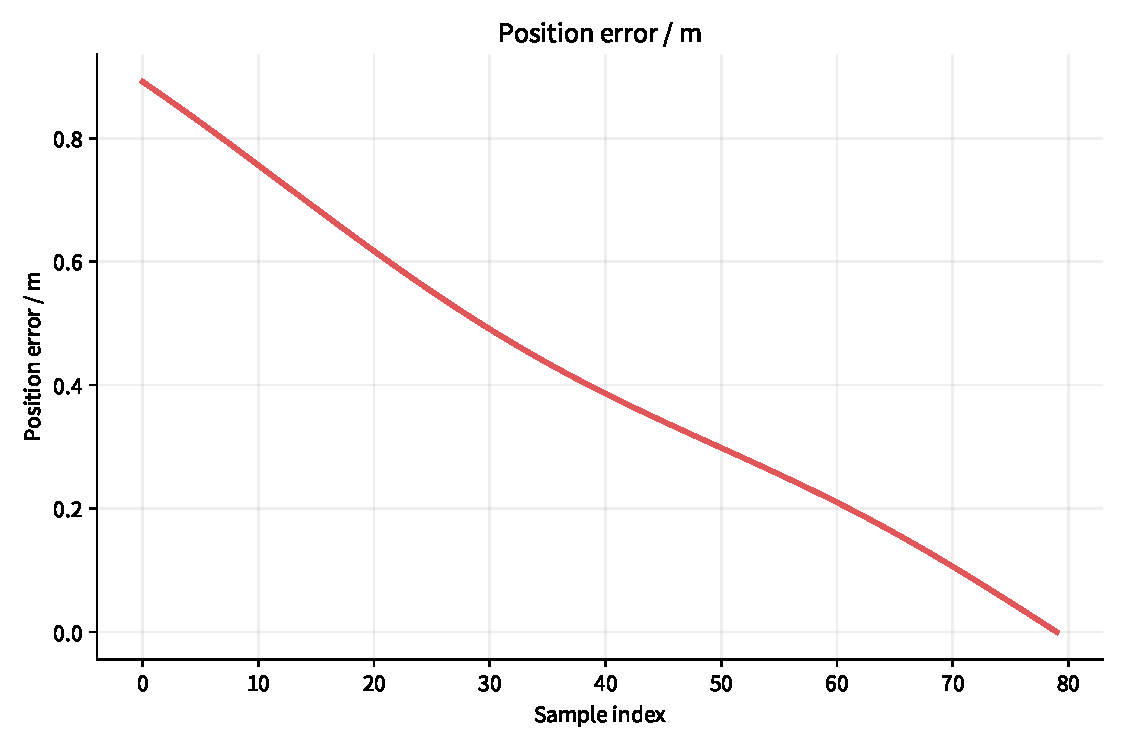
\includegraphics[width=0.82\linewidth,height=0.25\textheight,keepaspectratio]{generated/paper_ee_position_error.pdf}
  \caption{主展示轨迹的位置误差过程。该曲线用于观察末端是否稳定接近目标，而不是只在最后一个采样点满足阈值。}
  \label{fig:paper-ee-position-error}
\end{figure}

\begin{figure}[!htbp]
  \centering
  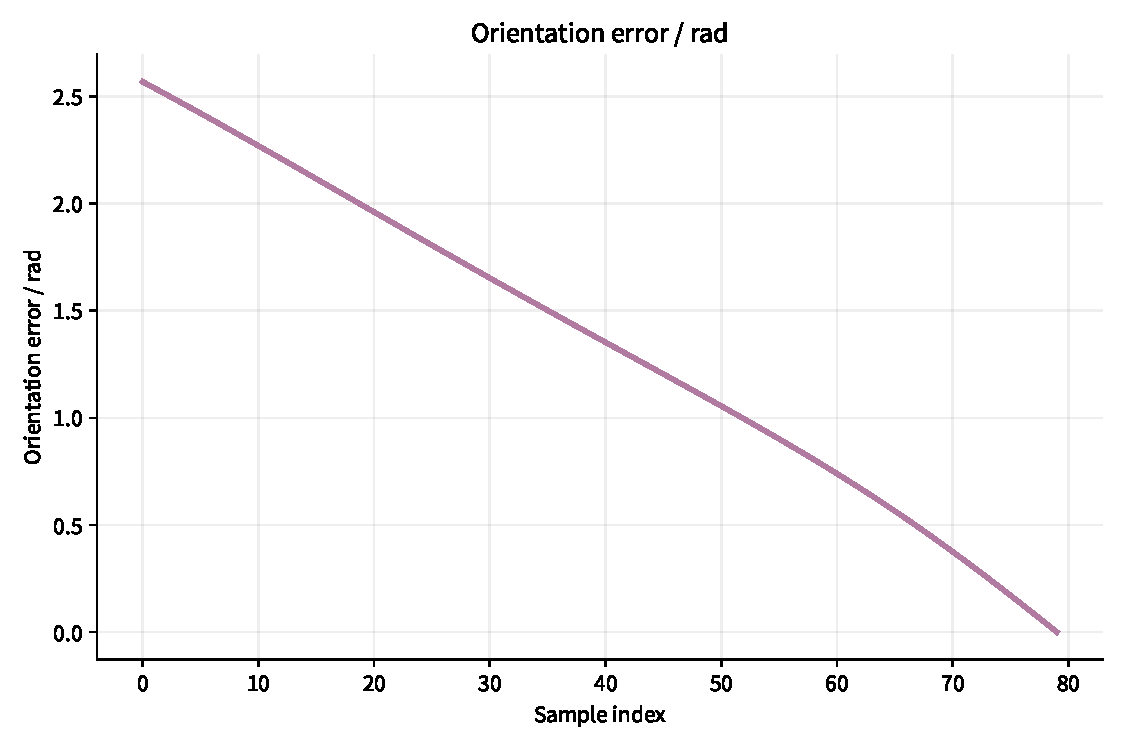
\includegraphics[width=0.82\linewidth,height=0.25\textheight,keepaspectratio]{generated/paper_ee_orientation_error.pdf}
  \caption{主展示轨迹的姿态误差过程。姿态误差以旋转向量范数表示，反映末端插入方向是否满足目标位姿要求。}
  \label{fig:paper-ee-orientation-error}
\end{figure}

\begin{figure}[!htbp]
  \centering
  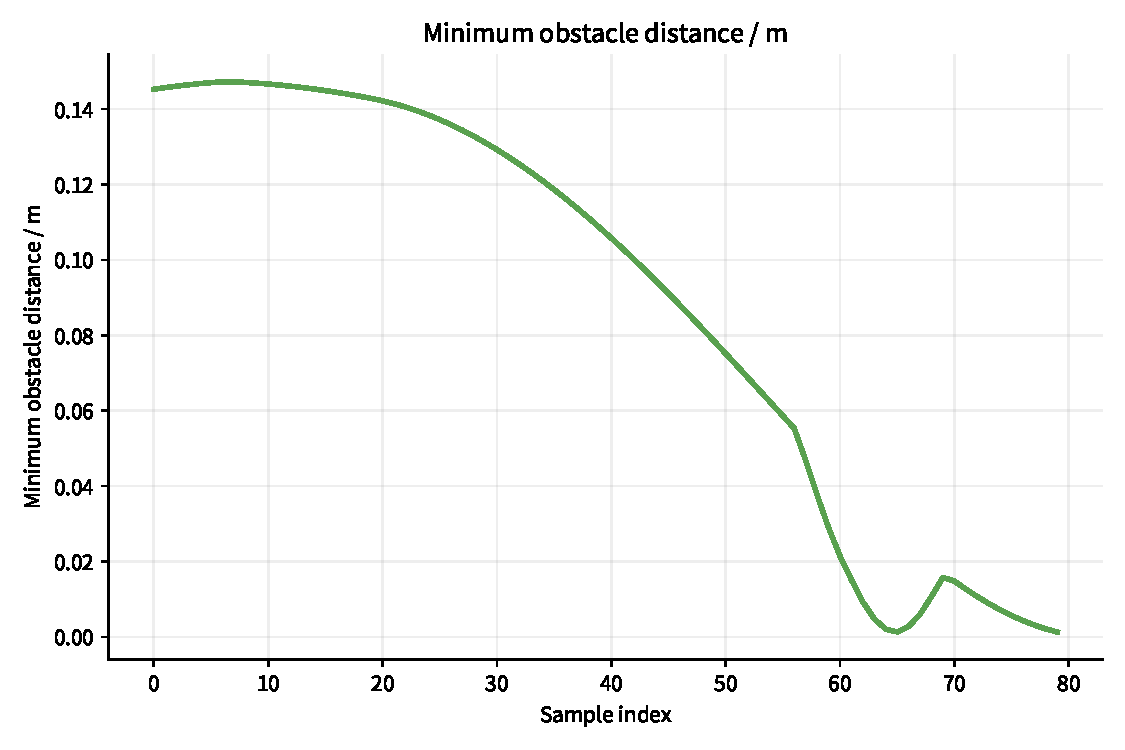
\includegraphics[width=0.82\linewidth,height=0.25\textheight,keepaspectratio]{generated/paper_min_obstacle_distance.pdf}
  \caption{主展示轨迹的最近障碍距离过程。该曲线越接近零，表示机械臂越贴近障碍物，安全裕度越小。}
  \label{fig:paper-min-obstacle-distance}
\end{figure}

\begin{figure}[!htbp]
  \centering
  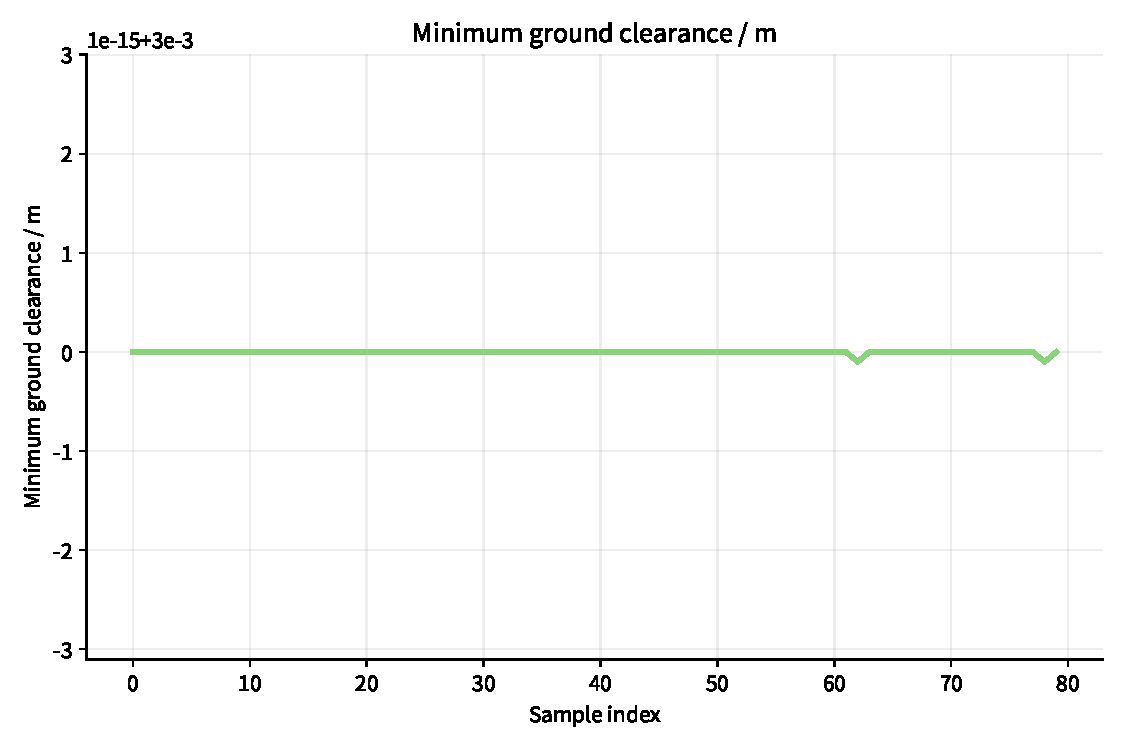
\includegraphics[width=0.82\linewidth,height=0.25\textheight,keepaspectratio]{generated/paper_min_ground_clearance.pdf}
  \caption{主展示轨迹的最小地面间隙过程。该图用于证明成功路径没有依赖穿过地面获得不可执行的捷径。}
  \label{fig:paper-min-ground-clearance}
\end{figure}

关节空间过程进一步描述轨迹平滑性。图 \ref{fig:paper-joint-speed-norm}、图 \ref{fig:paper-joint-acc-norm} 和图 \ref{fig:paper-joint-jerk-norm} 分别对应一阶、二阶和三阶差分范数。速度范数反映相邻采样点的关节变化幅度；加速度范数反映变化趋势是否平滑；jerk 范数则对高阶突变更敏感。若 jerk 曲线出现尖峰，即使路径无碰撞，也意味着后续真实控制器需要更强的时间参数化和平滑处理。

\begin{figure}[!htbp]
  \centering
  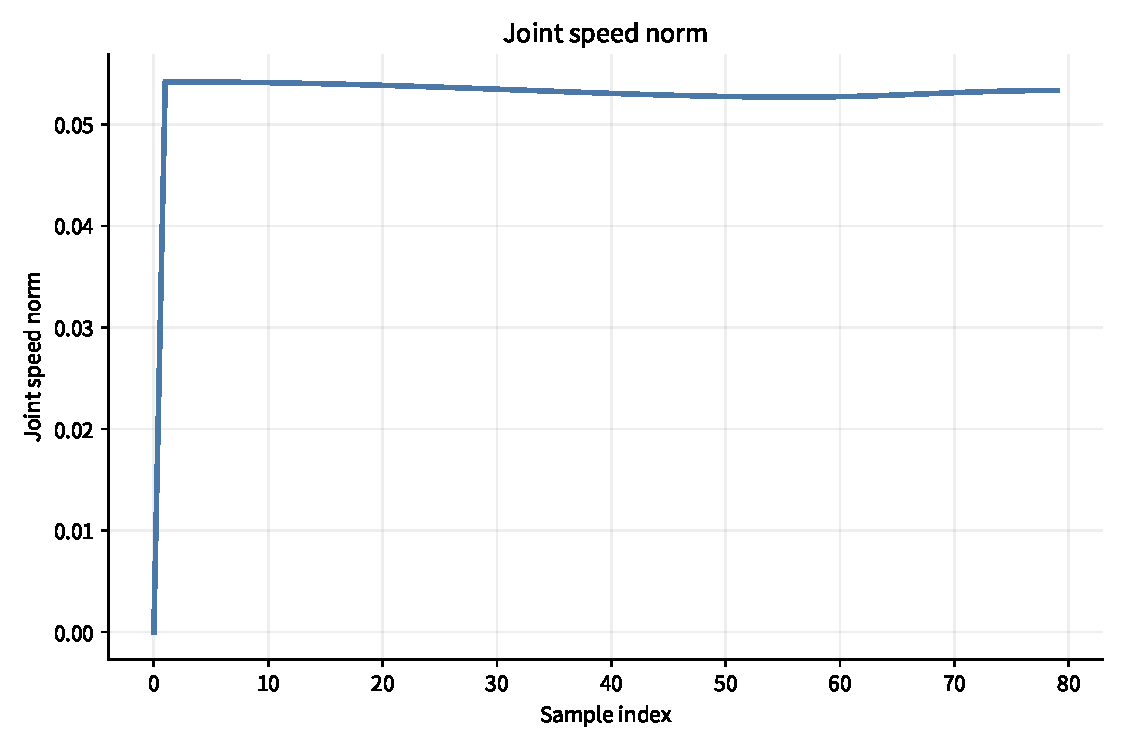
\includegraphics[width=0.82\linewidth,height=0.25\textheight,keepaspectratio]{generated/paper_joint_speed_norm.pdf}
  \caption{主展示轨迹的关节速度增量范数。该图反映相邻采样点之间关节空间变化是否均匀。}
  \label{fig:paper-joint-speed-norm}
\end{figure}

\begin{figure}[!htbp]
  \centering
  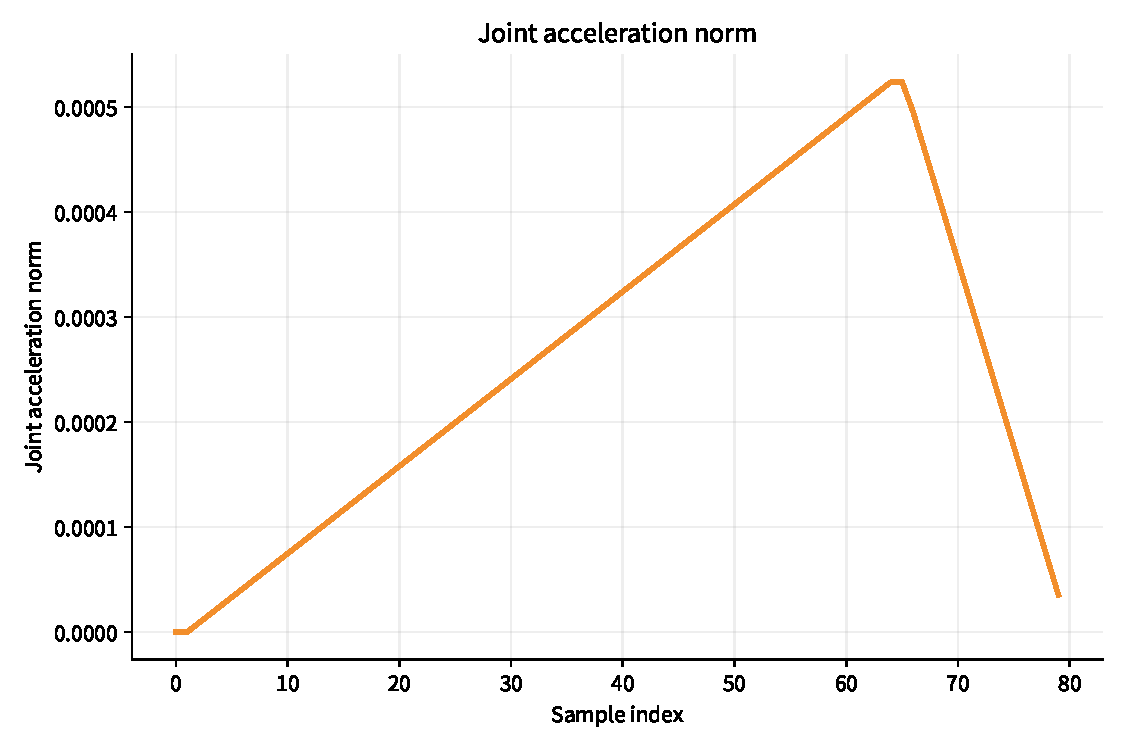
\includegraphics[width=0.82\linewidth,height=0.25\textheight,keepaspectratio]{generated/paper_joint_acc_norm.pdf}
  \caption{主展示轨迹的关节加速度差分范数。该图用于观察轨迹二阶变化是否平稳。}
  \label{fig:paper-joint-acc-norm}
\end{figure}

\begin{figure}[!htbp]
  \centering
  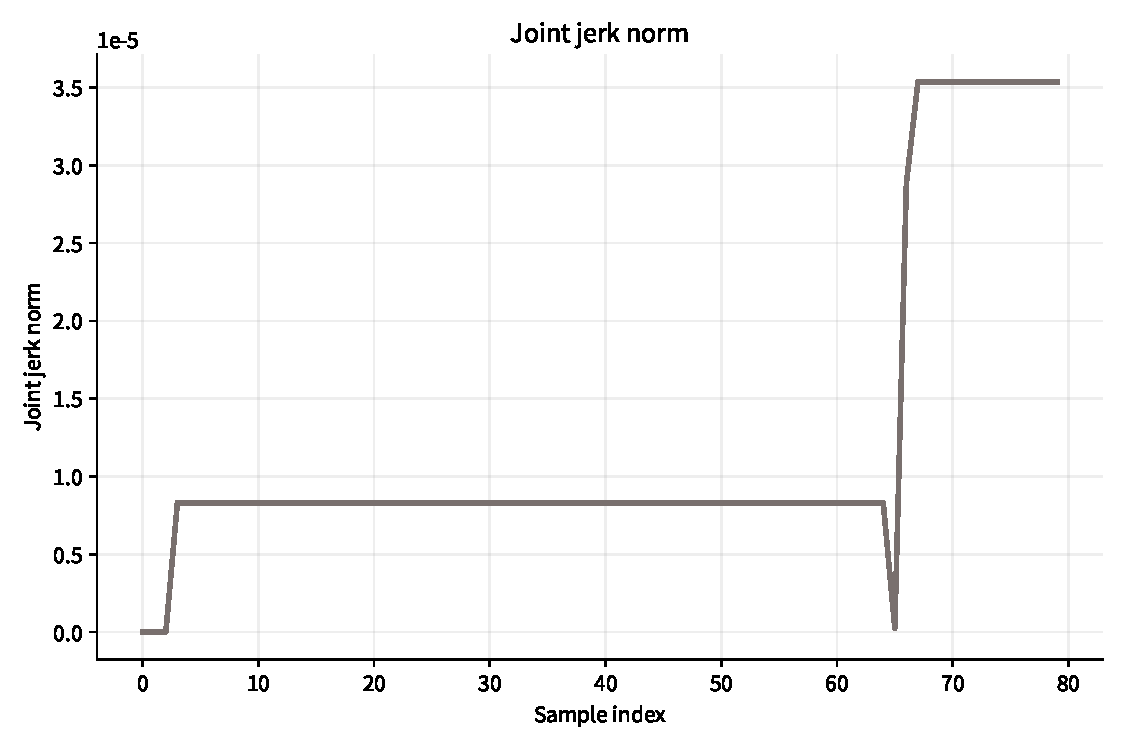
\includegraphics[width=0.82\linewidth,height=0.25\textheight,keepaspectratio]{generated/paper_joint_jerk_norm.pdf}
  \caption{主展示轨迹的关节 jerk 差分范数。该图用于检查高阶变化是否存在突发尖峰。}
  \label{fig:paper-joint-jerk-norm}
\end{figure}

\subsection{多场景成功与失败案例}
在前述基准场景之后，主展示场景用于综合呈现完整 UR5e 模型、位姿目标、密集悬浮障碍和地面约束下的成功案例。其成功轨迹如图 \ref{fig:paper-ee-path-3d-large} 和图 \ref{fig:paper-ee-path-top-view-large} 所示。三维图强调末端从悬浮障碍之间进入目标小框的空间过程，俯视图则更容易观察路径相对障碍中心线的横向偏移。两类图结合后，可以说明算法成功并不只是终点误差小，还需要轨迹在空间上满足避障、安全距离和地面间隙要求。

\begin{figure}[!htbp]
  \centering
  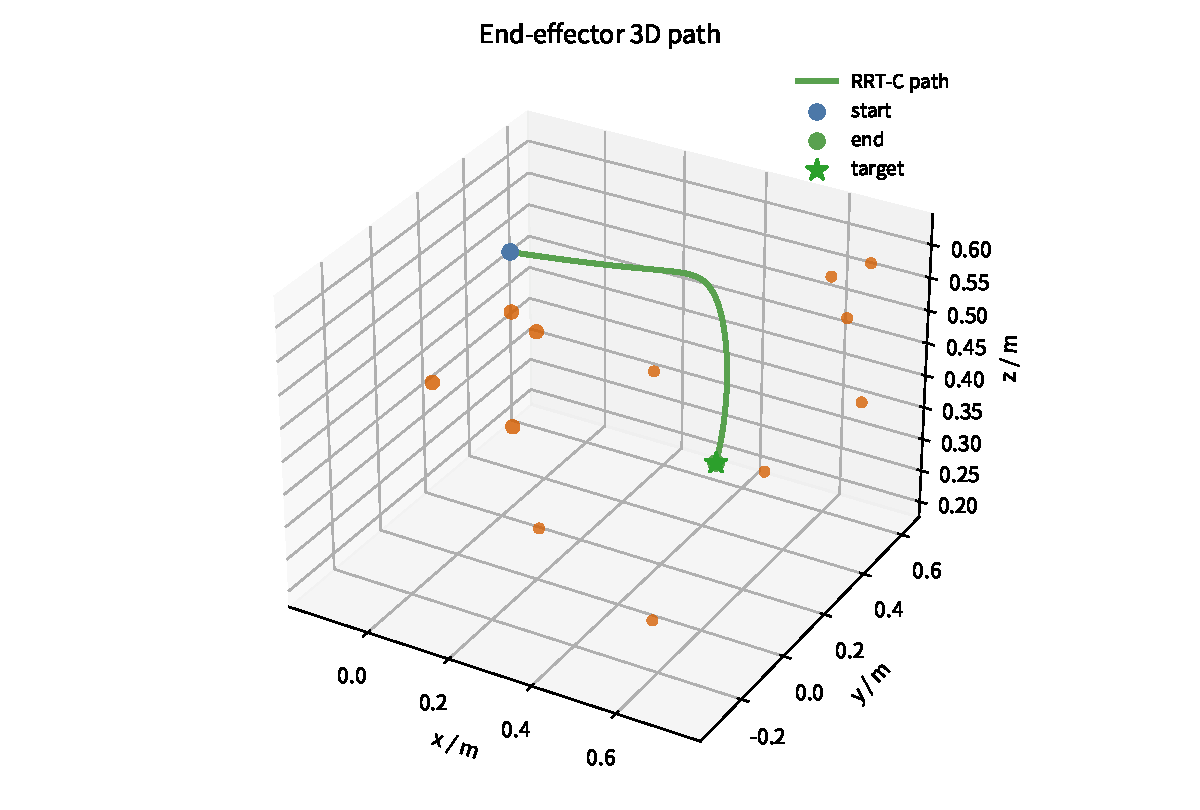
\includegraphics[width=0.88\linewidth,height=0.34\textheight,keepaspectratio]{generated/paper_ee_path_3d_large.pdf}
  \caption{主展示场景中的典型成功轨迹三维图。末端轨迹在密集悬浮障碍中接近目标小框，体现插入式目标到达过程。}
  \label{fig:paper-ee-path-3d-large}
\end{figure}

\begin{figure}[!htbp]
  \centering
  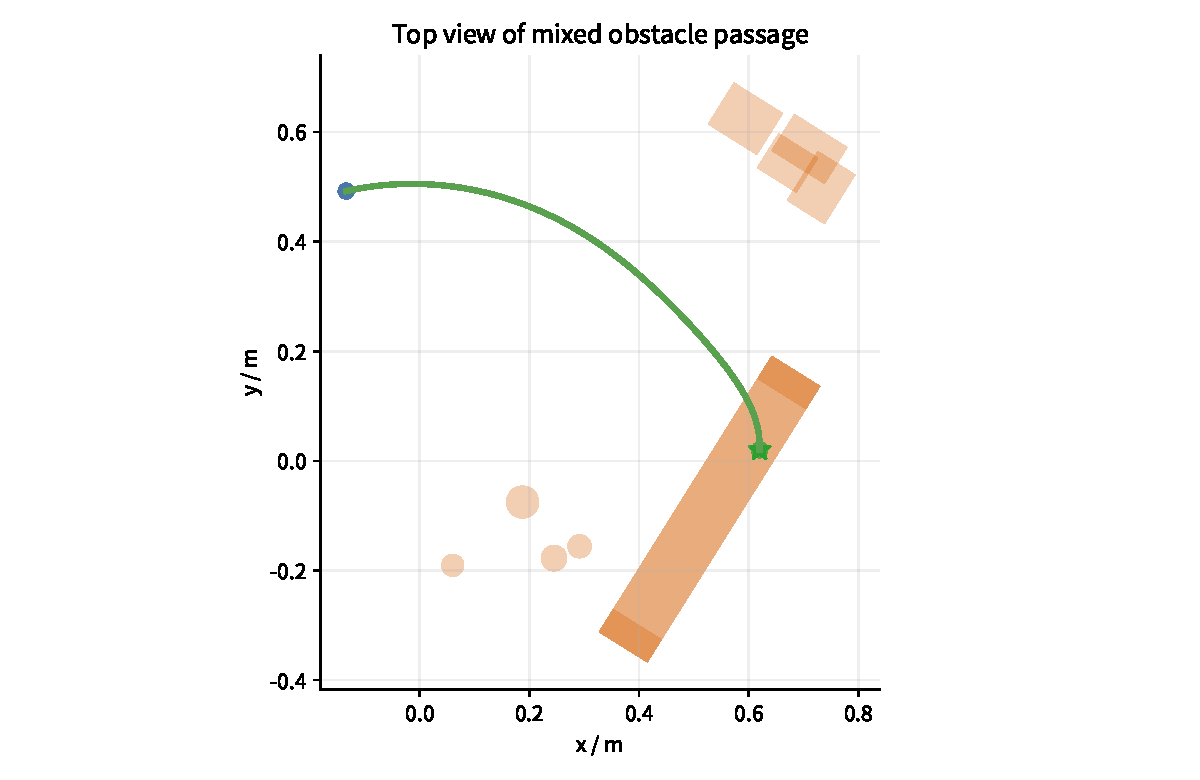
\includegraphics[width=0.88\linewidth,height=0.34\textheight,keepaspectratio]{generated/paper_ee_path_top_view_large.pdf}
  \caption{主展示场景中的典型成功轨迹俯视图。俯视投影用于观察轨迹是否从障碍间隙中通过，而不是从外围绕行。}
  \label{fig:paper-ee-path-top-view-large}
\end{figure}

失败场景主要来自三类机制。第一类是采样或连接不足，例如 RRT 在密集障碍中达到迭代上限，PRM 的路线图未连通；第二类是局部极小值，例如 APF 被吸引势和排斥势共同困住；第三类是物理约束失败，例如后处理轨迹发生碰撞或地面穿透。表 \ref{tab:failure-cases} 把这些失败类别和典型含义对应起来，图 \ref{fig:planner-failure-stacked} 给出统计数量，图 \ref{fig:mujoco-failure-snapshots} 则展示从失败 trial 中自动提取的 MuJoCo 瞬间构型。与只报告“失败”二字相比，失败快照能够直接观察末端离目标的剩余误差、机器人与障碍物的相对位置以及地面约束是否被触发。

\begin{table}[!htbp]
  \centering
  \caption{典型失败类别及其物理或数值含义}
  \label{tab:failure-cases}
  \small
  \begin{tabularx}{\textwidth}{p{3.4cm}X p{3.1cm}}
    \toprule
    失败类别 & 含义 & 常见算法 \\
    \midrule
    迭代上限 & 随机树或势场迭代次数耗尽，未能到达目标邻域。 & RRT、APF \\
    采样图未连通 & PRM 采样点或近邻边不足，起点和目标不在同一连通分量。 & PRM \\
    局部极小值 & 吸引势与排斥势抵消，梯度接近零但尚未到达目标。 & APF \\
    障碍碰撞 & 规划边或状态与障碍物几何体发生穿透。 & RRT、APF \\
    地面穿透 & 机器人几何体相对地面 plane 的距离小于 $-10^{-4}$ m。 & 后处理轨迹 \\
    后处理轨迹无效 & 原始路径成功，但 shortcut 或重采样后边插值复查失败。 & 所有规划器 \\
    \bottomrule
  \end{tabularx}
\end{table}

\begin{figure}[!htbp]
  \centering
  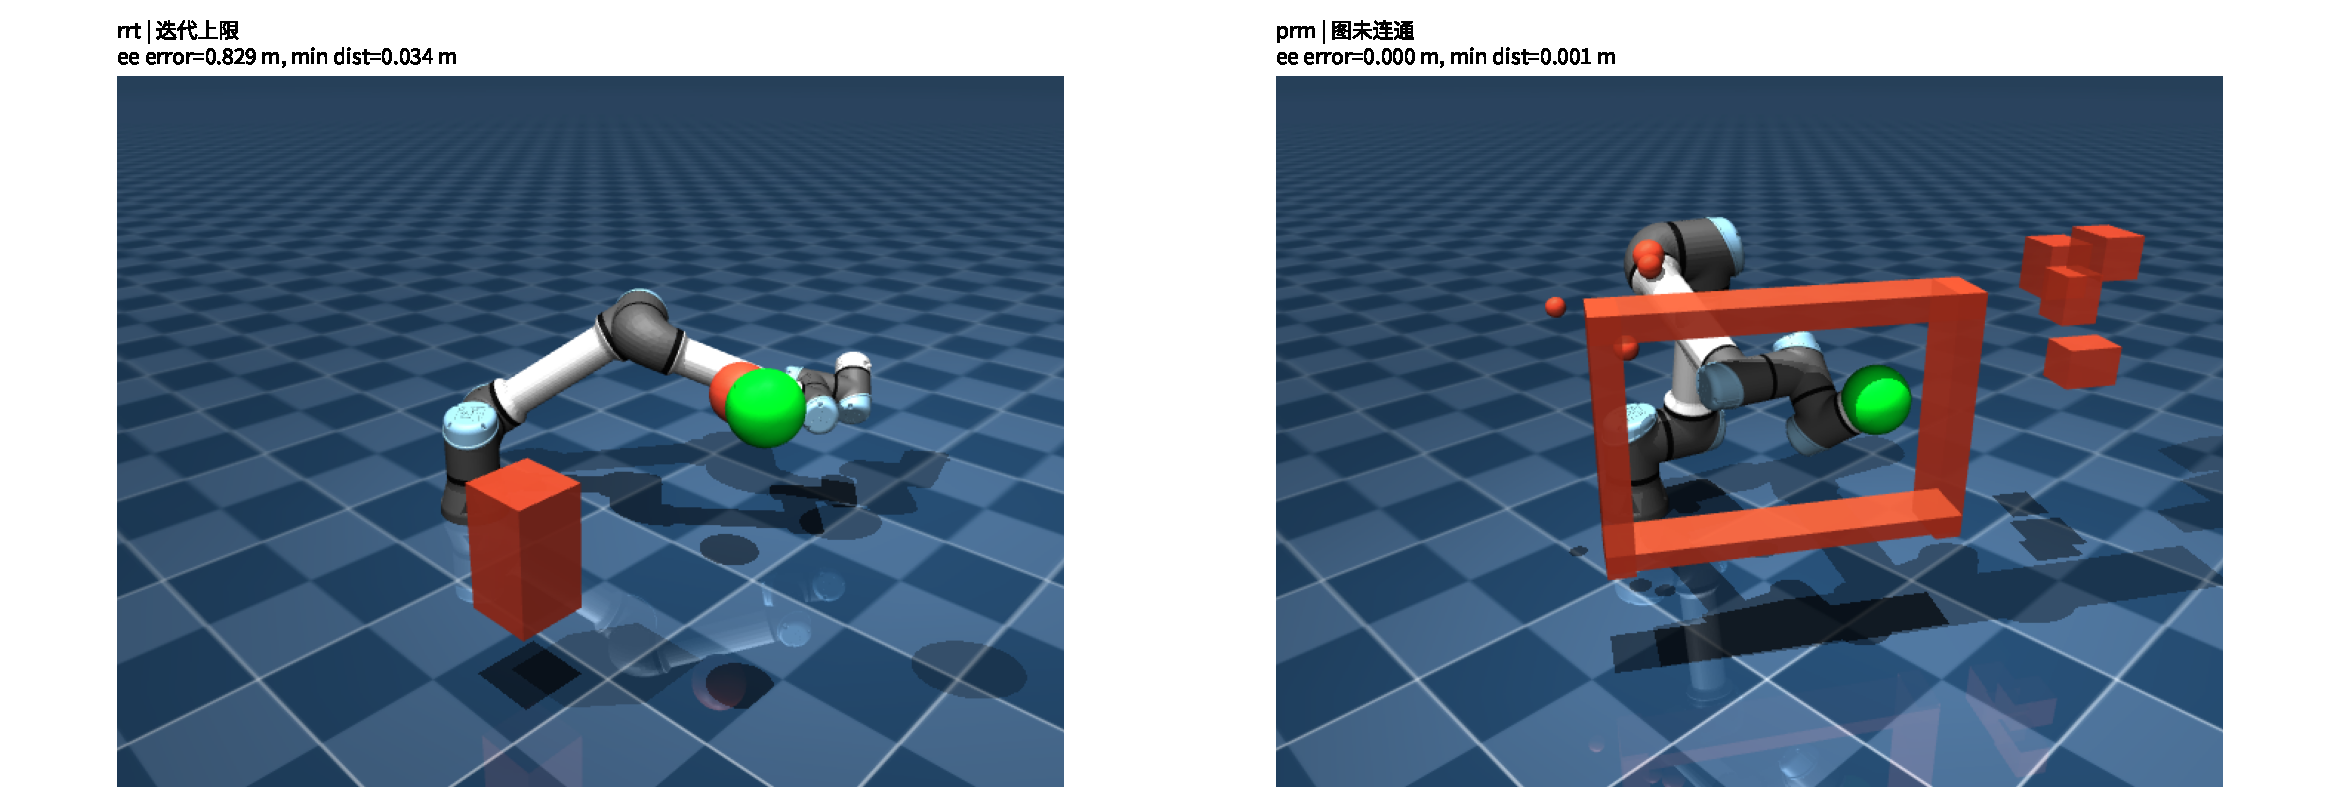
\includegraphics[width=0.90\linewidth,height=0.34\textheight,keepaspectratio]{generated/mujoco_failure_snapshots.pdf}
  \caption{典型失败瞬间的 MuJoCo 仿真画面。每个子图来自真实失败 trial 的代表构型，标题中给出规划器、失败类别、末端误差和最近障碍距离。}
  \label{fig:mujoco-failure-snapshots}
\end{figure}

\begin{figure}[!htbp]
  \centering
  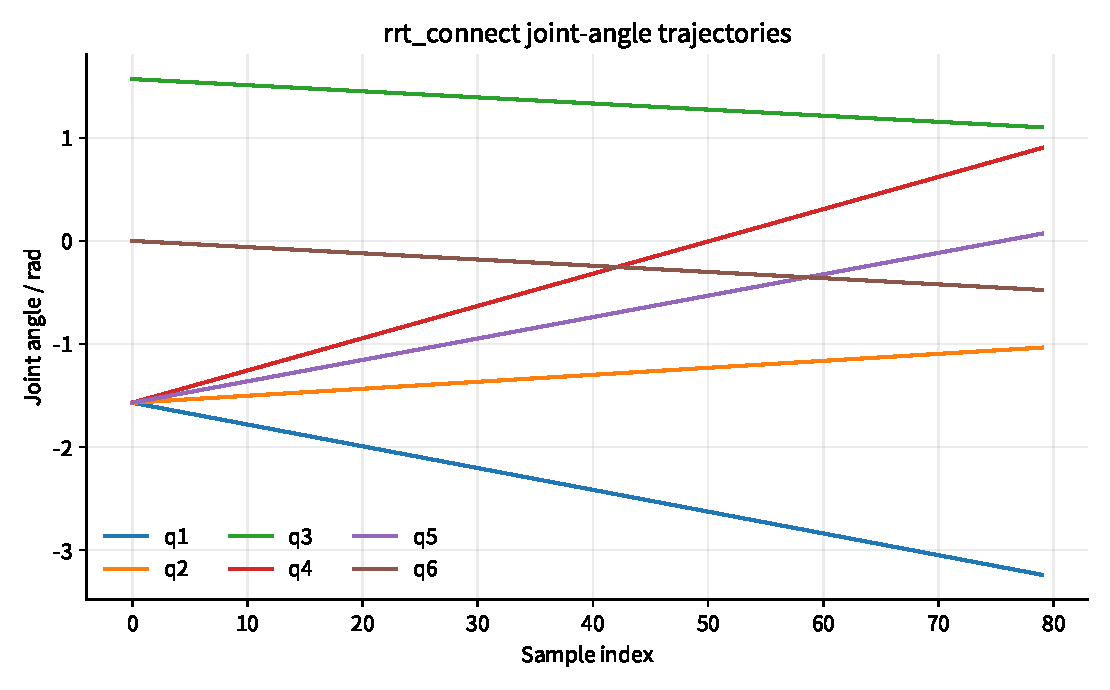
\includegraphics[width=0.88\linewidth,height=0.30\textheight,keepaspectratio]{generated/joint_angles_curve.pdf}
  \caption{RRT-Connect 成功轨迹的六关节角序列。该图用于检查各关节随采样点变化是否平滑且连续。}
  \label{fig:joint-angles-curve}
\end{figure}

\begin{figure}[!htbp]
  \centering
  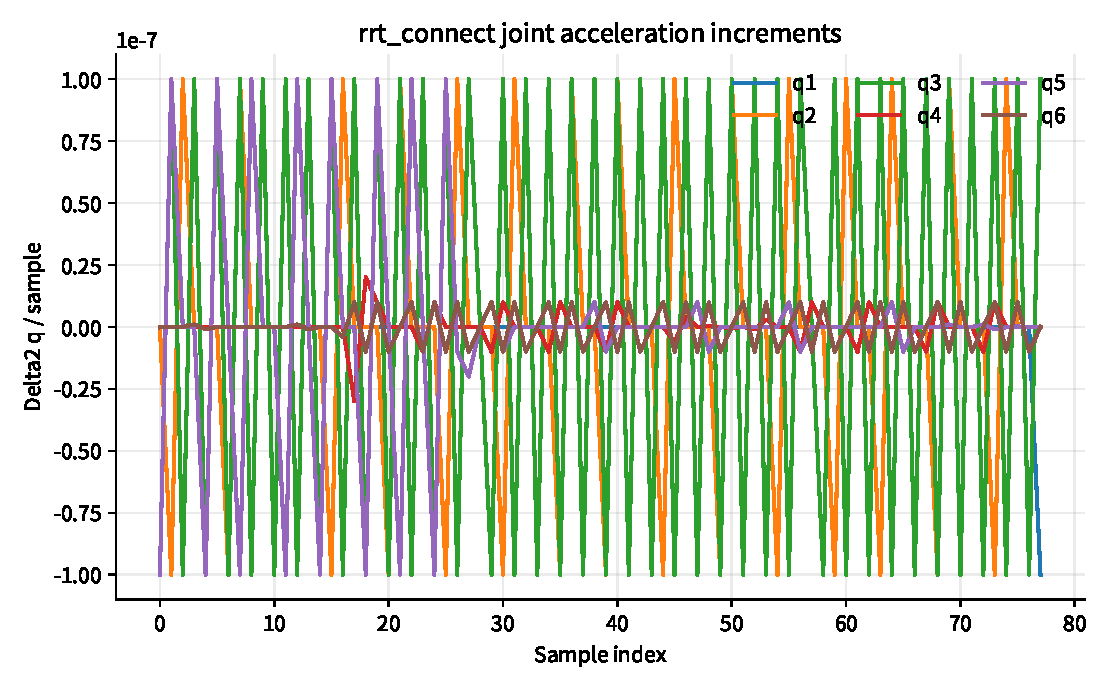
\includegraphics[width=0.88\linewidth,height=0.30\textheight,keepaspectratio]{generated/joint_acceleration_curve.pdf}
  \caption{RRT-Connect 成功轨迹的关节加速度差分。较小且连续的差分有助于说明轨迹具备更好的执行平滑性。}
  \label{fig:joint-acceleration-curve}
\end{figure}

\subsection{敏感性与误差来源}
本文结果受四个因素影响。第一是边检测分辨率。分辨率越小，越容易发现中间碰撞，但碰撞检测次数增加。第二是采样参数。RRT 类算法的步长和 goal bias 会影响探索速度，PRM 的样本数和邻居数会影响图连通性。第三是 MuJoCo 碰撞几何体近似。图 \ref{fig:mujoco-scene-no-obstacle}--图 \ref{fig:mujoco-scene-pass-through} 展示的是实际参与碰撞检测的几何体，而不是概念示意图；但完整 UR5e MJCF 模型仍以有限数量的 collision geom 表达真实机械臂外形，结果适合算法比较，不应直接等同于真实硬件部署性能。第四是地面穿透硬约束。该约束会降低表观成功率，却避免把物理上不可执行的穿地轨迹统计为成功。

从证据链角度看，MuJoCo 场景截图、末端轨迹图和 CSV 指标分别承担不同作用：场景截图说明障碍、地面和目标在空间中的真实布局；轨迹图说明末端如何穿过或绕开这些约束；CSV 指标则把位置误差、姿态误差、安全距离、地面间隙、速度、加速度和 jerk 量化下来。三者结合后，论文结论不再只依赖单一动画或单一数值表，而是同时具有空间可解释性和统计可复查性。

误差传播可概括为
\begin{equation}
  \delta\bm p
  \approx
  J(\bm q)\delta\bm q ,
  \label{eq:error-prop}
\end{equation}

因此
\begin{equation}
  \norm{\delta\bm q}_2
  \gtrsim
  \frac{\norm{\delta\bm p}_2}{\sigma_{\max}(J)} ,
  \label{eq:error-lower}
\end{equation}

而在接近奇异时
\begin{equation}
  \norm{\delta\bm q}_2
  \lesssim
  \frac{\norm{\delta\bm p}_2}{\sigma_{\min}(J)} .
  \label{eq:error-upper}
\end{equation}

这解释了为什么近奇异场景需要同时关注误差和条件数。

\subsection{工程使用建议}
若目标是交互式演示或在线避障，本文结果建议优先选择 DLS 或 LM 作为 IK 求解器，并使用 RRT-Connect 作为单次查询规划器。这个组合的优势不只来自成功率，还来自过程曲线：末端误差、姿态误差和障碍距离可以在有限采样点内保持可解释变化，且关节速度和 jerk 不会像失败的势场轨迹那样持续累积。

若目标是离线生成高精度目标构型，SciPy 最小二乘基线更适合作为参考解。它的代价是求解时间较长，因此不一定适合高频闭环。若工作环境固定且需要多次查询不同起终点，PRM 的前期构图成本可以被多次查询摊薄；但在本文单次任务比较中，这种优势没有完全体现。APF 的价值在于实现轻量和物理直观，适合作为局部修正或教学基线，但在复杂障碍、窄通道和小框插入场景中不宜作为唯一全局规划方法。

\section{结论}
本文基于 MuJoCo 与 Rerun 实现了一个可复现的六自由度机械臂避障路径规划数值实验平台，并将课程中的非线性方程组、线性化求解、条件数、插值、差分和采样近似统一到同一问题中。通过五个固定基准场景、一个完整 UR5e 主展示场景和每算法 50 次 trial，论文得到以下结论。

第一，逆运动学中 SciPy 最小二乘基线精度最高，但求解耗时约比阻尼 Jacobian 方法高一个数量级。DLS 和 LM 通过阻尼项改善了近奇异场景中的数值稳定性，适合作为实时性与稳定性折中的方法。

第二，路径规划中 RRT-Connect 在成功率、规划时间和碰撞检测次数上表现最均衡，是当前设置下最推荐的在线规划算法。PRM 成功率稳定但构图成本高，更适合多查询场景。RRT 简单有效，但在多障碍场景存在随机失败。APF 实现轻量，却容易受局部极小值影响。

第三，单一指标不足以判断规划质量。成功率说明是否可达，路径长度和耗时说明效率，安全距离说明碰撞裕度，速度、加速度和 jerk 说明执行平滑性。本文导出的 CSV、summary 表和图表使这些指标可以复查和复算。

综合算法优劣后，本文建议实时仿真展示优先采用 DLS 或 LM 生成目标构型，并配合 RRT-Connect 完成单次避障规划；离线高精度目标构型可采用 SciPy 最小二乘基线；固定环境中的多起终点查询可考虑 PRM；APF 则更适合作为轻量基线或局部修正模块，而不宜单独承担密集障碍场景下的全局规划。

后续工作可以从三个方向扩展：其一，把完整 UR5e 的碰撞几何体与真实控制器标定数据进一步对齐；其二，扫描边检测分辨率、RRT 步长和 PRM 样本数，形成更系统的敏感性曲线；其三，将 Rerun 记录与实际控制器接口连接，进一步验证规划轨迹的执行可行性。

\renewcommand{\refname}{参考文献}
\addcontentsline{toc}{section}{参考文献}
\bibliographystyle{ieeetr}
\bibliography{references}

\end{document}
